\documentclass[a4paper,12pt]{article}
\usepackage[T1]{fontenc}
\usepackage[utf8]{inputenc}
\usepackage[main=german,provide=*]{babel}
\usepackage{geometry}
\usepackage{graphicx}
\usepackage{float}
\usepackage{tabularx}
\usepackage[acronym]{glossaries}
\usepackage{hyperref}
\usepackage{parskip}
\newcommand{\captionwithsource}[2]{\caption{#1. Quelle: \url{#2}}}
\geometry{a4paper, margin=2.5cm}
\sloppy
\makeglossaries

%----------------------------------------------
% Glosar Einträge
%----------------------------------------------

\newglossaryentry{Frontend}{
  name        = Frontend,
  description = {Teil einer Anwendung, der für Nutzer sichtbar ist (Oberfläche, Benutzerinteraktion)}
}

\newglossaryentry{Backend}{
  name        = Backend,
  description = {Technischer Teil einer Anwendung, in dem Logik, Datenverarbeitung und Datenbanken laufen}
}

\newglossaryentry{Supabase}{
  name        = Supabase,
  description = {Cloud-basierte Backend-Plattform, die unter anderem Datenbanken, Authentifizierung und APIs bereitstellt}
}

\newglossaryentry{Vercel}{
  name        = Vercel,
  description = {Hosting-Plattform, die speziell auf moderne Webanwendungen wie z.\,B. Next.js ausgerichtet ist}
}

\newglossaryentry{Next.js}{
  name        = Next.js,
  description = {Framework für die Entwicklung von Webanwendungen mit React, inklusive Serverfunktionen}
}

\newglossaryentry{Prisma}{
  name        = Prisma,
  description = {ORM-Tool (Object-Relational Mapping), das den Zugriff auf Datenbanken vereinfacht}
}

\newglossaryentry{Merge-Konflikte}{
  name        = Merge-Konflikt,
  description = {Konflikt beim Zusammenführen von Änderungen im Code, wenn sich Änderungen widersprechen}
}

\newglossaryentry{Feature-Branches}{
  name        = Feature-Branch,
  description = {Separater Entwicklungszweig im Versionskontrollsystem (z.\,B. Git), in dem neue Funktionen entwickelt werden}
}

\newglossaryentry{Refactoring}{
  name        = Refactoring,
  description = {Umstrukturierung von Code, um ihn lesbarer, wartbarer oder effizienter zu machen, ohne Funktionalität zu ändern}
}

\newglossaryentry{Debugging}{
  name        = Debugging,
  description = {Systematisches Auffinden und Beheben von Fehlern im Code}
}

\newglossaryentry{Exploratory-Tests}{
  name        = Exploratory-Tests,
  description = {Freies Testen ohne feste Test-Skripte, um Schwachstellen oder unerwartetes Verhalten zu entdecken}
}

\newglossaryentry{Unit-Tests}{
  name        = Unit-Test,
  description = {Test auf kleinster Ebene, bei dem einzelne Funktionen oder Methoden isoliert überprüft werden}
}

\newglossaryentry{End-to-End-Tests}{
  name        = End-to-End-Test,
  description = {Test der gesamten Anwendung vom Start bis zur Benutzerinteraktion, um das Zusammenspiel aller Komponenten zu prüfen}
}

\newglossaryentry{Deployment}{
  name        = Deployment,
  description = {Veröffentlichung einer neuen Version der Anwendung auf einem Server oder einer Plattform}
}

\newglossaryentry{Balsamiq}{
  name        = Balsamiq,
  description = {Software-Tool zum schnellen Erstellen von Wireframes (visuelle Entwürfe von Benutzeroberflächen)}
}

\newglossaryentry{Upvote-Feature}{
  name        = Upvote-Feature,
  description = {Funktion, mit der Nutzer Inhalte (z.\,B. Wünsche) positiv bewerten können}
}

\newglossaryentry{In-App-Benachrichtigungen}{
  name        = In-App-Benachrichtigungen,
  description = {Direkt in der Anwendung angezeigte Hinweise oder Mitteilungen für die Nutzer}
}

\newglossaryentry{TypeScript}{
  name        = TypeScript,
  description = {Typsichere Programmiersprache, die auf JavaScript basiert und häufig in modernen Webanwendungen eingesetzt wird}
}

\newglossaryentry{React}{
  name        = React,
  description = {JavaScript-Bibliothek zur Erstellung von Benutzeroberflächen, insbesondere für Single-Page-Applications}
}

\newglossaryentry{Docker}{
  name        = Docker,
  description = {Plattform zur Containerisierung von Anwendungen zur Sicherstellung von portabler und konsistenter Laufzeitumgebung}
}

\newglossaryentry{JWT}{
  name        = JWT,
  description = {JSON Web Token – Kompakt formatierter Token zur sicheren Übertragung von Informationen zwischen Parteien als JSON-Objekt}
}

\newglossaryentry{REST}{
  name        = REST,
  description = {Architekturstil für Webservices, der auf HTTP-Protokollen basiert und CRUD-Operationen unterstützt}
}

\newglossaryentry{CRUD}{
  name        = CRUD,
  description = {Abkürzung für Create, Read, Update, Delete – Grundoperationen auf Daten in Webanwendungen}
}

\newglossaryentry{API}{
  name        = API,
  description = {Abkürzung für Application Programming Interface Schnittstelle, die es ermöglicht, Funktionen und Daten eines Softwaresystems von außen programmgesteuert zu nutzen}
}



\begin{document}

%----------------------------------------------
% Deckblatt
%----------------------------------------------

\begin{titlepage}
    \centering

    \vspace*{1.5cm}

    {\LARGE\bfseries Event-Planer\par}
    \vspace{0.3cm}
    {\normalsize Webapplikation zur Planung und Durchführung interner Events\par}

    \vspace{0.5cm}

    \begin{figure}[H]
        \centering
        
\includegraphics[width=0.35\textwidth]{Abbildungen/logo.png}
        \caption{Logo Event-Planer}
        \label{fig:logo}
        {\footnotesize Quelle: \url{https://chatgpt.com/s/m_685af32608c4819195bb875081578cd1}}
    \end{figure}

    \vspace{1.2cm}

    {\normalsize
    \begin{tabular}{rl}
        \textbf{Projektteam:}      & Felix Hoffmann \\
                                   & Baran Bickici \\
                                   & Sami Gökpinar \\
                                   & Ergün Bickici \\[0.5em]
        \textbf{Partnerunternehmen:} & pep.digital \\[0.5em]
        \textbf{Studiengang:}      & Softwaretechnik und Medieninformatik \\
                                   & 4. Semester, Sommersemester 2025 \\[0.5em]
        \textbf{Kunde:}            & Alexander Brendel \\[0.5em]
        \textbf{Betreuer:}         & Klemens Morbe \\[0.5em]
        \textbf{GitHub-Repository} & \url{https://github.com/pndroa/event-planer}
    \end{tabular}
    }

    \vfill
    {\small \today}
\end{titlepage}


\newpage

%----------------------------------------------
% Inhaltsverzeichnis
%----------------------------------------------

\tableofcontents

\newpage

%----------------------------------------------
% Abbildungsverzeichnis
%----------------------------------------------
\listoffigures

\newpage

%----------------------------------------------
% Tabellenverzeichnis
%----------------------------------------------
\listoftables

\newpage

%----------------------------------------------
% 1. Einführung
%----------------------------------------------

\section{Einführung}
Im Rahmen des Softwareprojekts im 4. Semester des Studienganges Softwaretechnik und Medieninformatik wird über das ganze Semester ein Projekt mit einem Partnerunternehmen, die als Kunden agieren durchgeführt. Dieses Projekt wird mit dem Unternehmen pep.digital die sich ein Produkt wünschen mit dem Titel "Event-Planer". Dieses Produkt soll eine Web-Applikation werden, in denen Mitarbeiter des Unternehmen pep.digital Events erstellen und das Event planen können z.B. mit Umfragen, Datum des Events und Teilnehmer. Dazu hat man auch die Möglichkeit Wünsche zu äußern aus denen man Events erstellen kann. Als erstes wird sich erst auf Schulungsevents konzentriert und in der Zukunft hat man die Möglichkeit auch andere Arten von Events zu erstellen.

%----------------------------------------------
% 2. Technologien
%----------------------------------------------

\section{Technologien}

%----------------------------------------------
% 2.1 Full-Stack-Framework
%----------------------------------------------

\subsection{Full-Stack Framework}
Für die Umsetzung des Projekts wurde \gls{Next.js} als Full-Stack-Framework gewählt. Next.js basiert auf \gls{React} und bietet eine vollständige Lösung für die Entwicklung von Webanwendungen, indem es sowohl Frontend- als auch Backend-Funktionalitäten integriert. Mit Next.js können Entwickler sowohl serverseitiges Rendering (SSR) als auch statische Seitengenerierung (SSG) nutzen. Zudem bietet es eine einfache Möglichkeit, API-Routen zu erstellen, was es zu einer hervorragenden Wahl für Full-Stack-Entwicklungen macht. Die Verwendung von \gls{TypeScript} sorgt für eine typsichere und fehlerarme Entwicklung, sowohl im \gls{Frontend} als auch im Backend.

%----------------------------------------------
% 2.1.1 Frontend
%----------------------------------------------

\subsubsection{Frontend}
Im Frontend nutzt Next.js React. React ist eine quelloffene JavaScript-Bibliothek, die das Erstellen der Benutzeroberfläche schnell und dynamisch macht. Anhand von React können Web- und Mobile-Anwendungen mit derselben Codebasis erstellt werden, ohne jegliche Formatierung. Die Codierung erfolgt in TypeScript, was durch statische Typisierung und bessere Fehlererkennung das Entwickeln sicherer und effizienter macht.

%----------------------------------------------
% 2.1.2 Backend
%----------------------------------------------

\subsubsection{Backend}
Das \gls{Backend} in Next.js wird durch das integrierte API-Routing realisiert, das auf Node.js basiert. Durch diese Integration können Entwickler API-Routen direkt innerhalb der Next.js-Anwendung erstellen, ohne einen separaten Server benötigen zu müssen. Diese Routen ermöglichen es, serverseitige Logik auszuführen, wie etwa das Abrufen von Daten aus einer Datenbank oder das Bearbeiten von Anfragen. Da Next.js auf Node.js aufbaut, können alle leistungsfähigen Funktionen von Node.js genutzt werden, während TypeScript die Entwicklung durch statische Typisierung und Fehlererkennung verbessert. Dies sorgt für eine konsistente und sichere Entwicklung sowohl im Frontend als auch im Backend innerhalb derselben Codebasis.

\newpage

%----------------------------------------------
% 2.2 Datenbank
%----------------------------------------------

\subsection{Datenbank}
Für die Umsetzung der Anwendung wurde eine relationale Datenbank auf Basis von PostgreSQL gewählt. Diese Entscheidung basiert auf der strukturellen Beschaffenheit der Daten sowie auf Vorkenntnissen im Umgang mit relationalen Datenbanksystemen. Die Anwendung verarbeitet klar strukturierte Daten wie Nutzerinformationen, Veranstaltungsdetails, Wunschvorschläge und Umfrageergebnisse. Viele dieser Entitäten weisen ähnliche Attribute auf oder stehen in logisch definierten Beziehungen zueinander. Relationale Datenbanken eignen sich in solchen Szenarien besonders gut, da sie eine eindeutige Abbildung von Beziehungen ermöglichen. Zudem liegen bereits umfangreiche Erfahrungen im Umgang mit relationalen Datenbanken vor, unter anderem durch vergangene Vorlesungen und Projekte mit SQL. Der Einsatz einer vertrauten Technologie ermöglicht eine effizientere Umsetzung des Datenmodells, ohne zusätzlichen Einarbeitungsaufwand in alternative Datenbankkonzepte. PostgreSQL wurde als Datenbankmanagementsystem gewählt, da es als stabile und gut dokumentierte Lösung gilt. Es deckt sowohl grundlegende Anforderungen wie CRUD-Operationen als auch komplexere Anforderungen hinsichtlich Datenintegrität ab. In Kombination mit der Backend as a Service Plattform \gls{Supabase} wird die Datenbank um Zugriffskontrollen ergänzt, ohne dass dafür viel eigene Backend-Logik nötig ist.

%----------------------------------------------
% 2.3 Authentifizierung
%----------------------------------------------

\subsection{Authentifizierung}
Supabase wird für die Authentifizierung genutzt, da es eine einfache und sichere Möglichkeit bietet, Nutzer in eine Anwendung zu integrieren. Es unterstützt Single Sign-On (SSO) und externe Identitätsanbieter wie Google und Microsoft Azure, sodass sich Benutzer bequem mit ihren bestehenden Konten anmelden können. Durch die Integration von Microsoft Azure können sich insbesondere Mitarbeiter direkt mit ihren Microsoft-Accounts authentifizieren. Dies erleichtert den Zugriff auf die Anwendung, da keine separaten Anmeldeinformationen erstellt werden müssen, und sorgt gleichzeitig für höhere Sicherheit und bessere Verwaltungsmöglichkeiten durch zentrale Benutzerkontrollen in Azure.

%----------------------------------------------
% 2.4 Bereitstellung
%----------------------------------------------

\subsection{Bereitstellung}
Zur Bereitstellung wird in diesem Projekt \gls{Docker} verwendet, da so sicher gegangen werden kann, dass die Anwendung in einer konsistenten Umgebung ausgeführt wird, unabhängig von den zugrunde liegenden Betriebssystemen oder Hardwarekonfigurationen.

\newpage

%----------------------------------------------
% 3. Anforderungsspezifikation
%----------------------------------------------

\section{Anforderungsspezifikation}

%----------------------------------------------
% 3.1 Zielgruppe
%----------------------------------------------

\subsection{Zielgruppe}
Mit dem Endprodukt des Projekts, wird den Mitarbeitenden des Unternehmen pep.digital eine Web-Applikation für die Erstellung und Planung von Events zur Verfügung gestellt. Da diese Web-Applikation firmenspezifisch und  nicht für den offenen Markt entwickelt wird, ist die Zielgruppe dieser App sehr reduziert. Dies bedeutet im Umkehrschluss, dass ähnliche Applikationen und Konkurrenten bei der Entwicklung dieser App keine Rolle spielen. Durch die Analyse bereits bestehender Anwendungen, wurden gelungene Eigenschaften und Makel aufgelistet. Dadurch ist klar, worauf es bei der Entwicklung geachtet werden soll

%----------------------------------------------
% 3.2 Kundenbefragung
%----------------------------------------------

\subsection{Kundenbefragung}
Eine Kundenbefragung bei der Softwareentwicklung ist wichtig, um die Bedürfnisse und Erwartungen der Zielgruppe zu verstehen. Durch direktes Feedback von potenziellen Nutzern können Entwickler ihre Produkte besser anpassen und optimieren. Im Gespräch mit dem Kunden ergaben sich beispielsweise Informationen über den Prozess der Erstellung der Events und Wünsche.

%----------------------------------------------
% 3.3 Feature-Map
%----------------------------------------------

\subsection{Feature-Map}
Aus der Kundenbefragung ergab sich diese Feature-Map:
\begin{figure}[H]
    \centering
    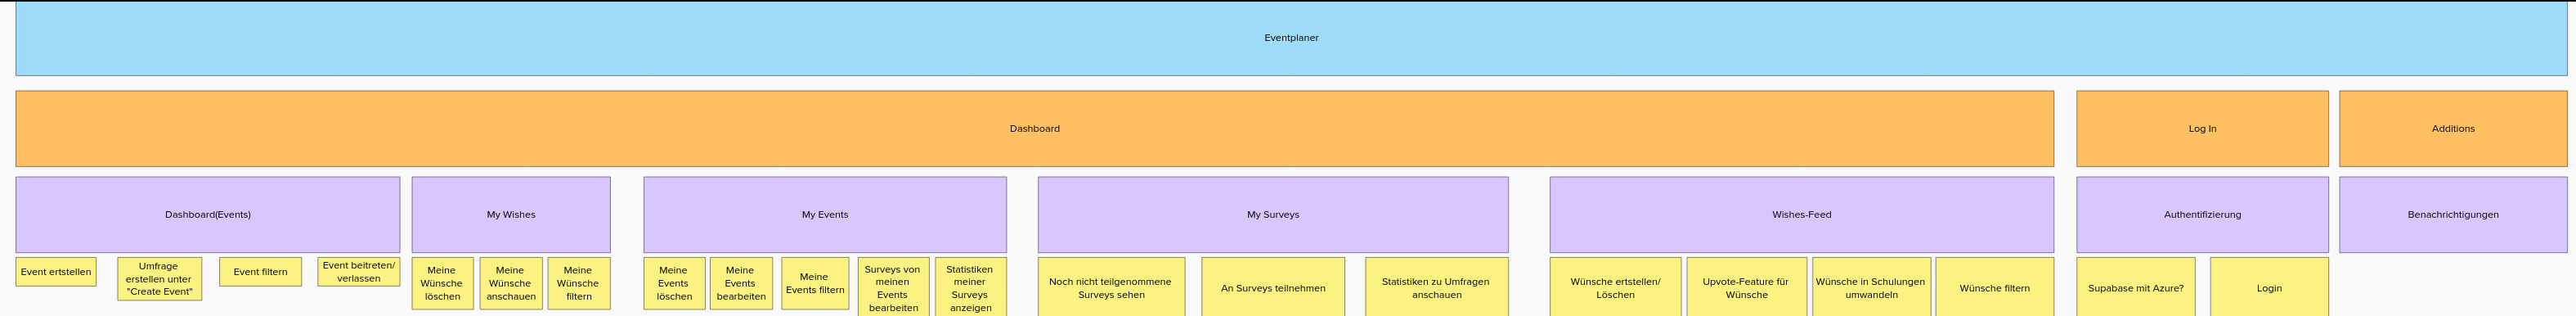
\includegraphics[width=1\textwidth]{Abbildungen/feature_map.png}
    \caption{Feature-Map}
    \label{fig:feature_map}
\end{figure}

\newpage

%----------------------------------------------
% 3.4 User Stories
%----------------------------------------------

\subsection{User Stories}

%----------------------------------------------
% 3.4.1 Anmeldung
%----------------------------------------------

\subsubsection{Anmeldung}
\begin{itemize}
  \item \textbf{Als Benutzer}, möchte ich mich mit einem bestehenden Account (z.B. Microsoft) anmelden können, \textbf{damit ich} mich nicht neu registrieren muss und die Applikation direkt mit meinem persönlichen Profil nutzen kann.
  \item \textbf{Als Benutzer} möchte ich mich mit meiner eigenen E-Mail-Adresse und einem selbstgewählten Passwort registrieren können, \textbf{damit ich} ein individuelles Benutzerkonto erstellen und die Applikation nutzen kann.
  \item \textbf{Als Benutzer} möchte ich mich mit meiner bei der Registrierung erstellten E-Mail-Adresse und meinem Passwort anmelden können, \textbf{damit ich} auf mein persönliches Benutzerkonto in der Applikation zugreifen kann.
\end{itemize}

%----------------------------------------------
% 3.4.1 Events
%----------------------------------------------

\subsubsection{Events}
\begin{itemize}
  \item \textbf{Als Benutzer} möchte ich Events erstellen können, \textbf{damit ich} eigene Veranstaltungen organisieren und veröffentlichen kann, die für alle Nutzer sichtbar sind.
  \item \textbf{Als Benutzer} möchte ich eine Übersichtsseite mit allen geplanten Events sehen können, \textbf{damit ich} schnell einen Überblick über bevorstehende Veranstaltungen erhalte und mich bei Interesse direkt dafür anmelden kann.
  \item \textbf{Als Benutzer} möchte ich einem Event beitreten können, \textbf{damit ich} meine Teilnahme an Veranstaltungen bestätigen und sicherstellen kann, dass ich für das Event registriert bin.
  \item \textbf{Als Benutzer} möchte ich ein Event, dem ich bereits beigetreten bin, wieder verlassen können, \textbf{damit ich} meine Teilnahme zurückziehen kann, falls ich doch nicht an der Veranstaltung teilnehmen kann.
  \item \textbf{Als Veranstalter} möchte ich Events, die ich erstellt habe, bearbeiten können, \textbf{damit ich} Informationen wie Titel, Datum oder Beschreibung aktualisieren und Änderungen an der Veranstaltung kommunizieren kann.
  \item \textbf{Als Veranstalter} möchte ich Events, die ich selbst erstellt habe, löschen können, \textbf{damit ich} fehlerhafte oder nicht mehr relevante Veranstaltungen aus dem System entfernen kann.
\end{itemize}

%----------------------------------------------
% 3.4.2 Wünsche
%----------------------------------------------

\subsubsection{Wünsche}
\begin{itemize}
  \item \textbf{Als Benutzer} möchte ich einen Wunsch für eine Veranstaltung zu einem bestimmten Thema erstellen können, \textbf{damit ich} Vorschläge für neue Events einbringen kann.
  \item \textbf{Als Benutzer} möchte ich eigene erstellte Wünsche wieder löschen können, \textbf{damit ich} nicht mehr relevante oder falsch erstellte Wünsche entfernen kann
  \item \textbf{Als Benutzer} möchte ich Wünsche anderer Nutzer upvoten können, \textbf{damit ich} Interesse an vorgeschlagenen Veranstaltungen zeigen und unterstützen kann, dass diese umgesetzt werden.
  \item \textbf{Als Veranstalter} möchte ich mich zu einem Wunsch bereitstellen und daraus ein neues Event erstellen können, \textbf{damit ich} gezielt Veranstaltungen nach den Interessen der Nutzer anbieten kann.
\end{itemize}

%----------------------------------------------
% 3.4.3 Umfragen
%----------------------------------------------

\subsubsection{Umfragen}
\begin{itemize}
  \item \textbf{Als Veranstalter} möchte ich innerhalb eines Events eine Umfrage für die Teilnehmer erstellen können, \textbf{damit ich} Feedback oder Meinungen zu bestimmten Themen einholen kann
  \item \textbf{Als Veranstalter} möchte ich eine von mir erstellte Umfrage bearbeiten können, \textbf{damit ich} Fragen oder Antwortoptionen anpassen kann, bevor die Umfrage abgeschlossen ist.
  \item \textbf{Als Veranstalter} möchte ich bei jedem Event die statistischen Auswertungen der Umfragen einsehen können, \textbf{damit ich} schnell einen Überblick darüber bekomme, zu welchen Optionen oder Themen die meisten Teilnehmer tendieren.
  \item \textbf{Als Benutzer} möchte ich einen Bereich haben, in dem ich alle meine noch nicht abgeschlossenen Umfragen sehen kann, \textbf{damit ich} den Überblick über offene Umfragen behalte und diese bei Bedarf weiterbearbeiten oder abschließen kann.
\end{itemize}

\newpage

%----------------------------------------------
% 4. Funktionsumfang
%----------------------------------------------

\section{Funktionsumfang}
Der Funktionsumfang vom Event-Planer wurde sorgfältig entwickelt, um eine umfassende und benutzerfreundliche Erfahrung für Mitarbeitende der Unternehmen pep.digital zu gewährleisten. Im Folgenden sind die Hauptfunktionen im Detail aufgeführt:

%----------------------------------------------
% 4.1 Anmeldung und Registrierung
%----------------------------------------------

\subsection{Anmeldung und Registrierung}
Mitarbeitende können sich mühelos mit ihrem bestehenden Unternehmensaccount über Microsoft anmelden. Die benutzerfreundliche und intuitive Oberfläche optimiert den Anmeldeprozess. Zusätzlich haben auch externe Nutzer die Möglichkeit, sich unabhängig vom Unternehmen zu registrieren.

%----------------------------------------------
% 4.2 Events
%----------------------------------------------

\subsection{Events}
User haben die Möglichkeit, eigene Events zu erstellen, zu bearbeiten und zu löschen. Jedes Event umfasst einen Titel und eine Beschreibung, in der Details zur Veranstaltung festgehalten werden können. Nach der Erstellung können Events jederzeit vom Ersteller angepasst werden, sei es zur Änderung des Titels, der Beschreibung oder weiterer relevanter Informationen. Falls ein Event nicht mehr benötigt wird, kann es auch gelöscht werden. Für eine bessere Übersicht gibt es einen \textbf{Event-Feed}, in dem alle Events angezeigt werden. Hier können User schnell durch die verschiedenen Veranstaltungen stöbern und sich inspirieren lassen. Zudem gibt es eine eigene Sektion \textbf{„Meine Events“}, in der User ihre eigenen erstellten Events verwalten können. Hier können sie ihre Events ansehen, bearbeiten oder löschen. Nach dem Event können individuelle Umfragen erstellt und jederzeit vom Ersteller bearbeitet werden. Diese Umfragen dienen dazu, Feedback und Meinungen der Teilnehmer zu sammeln. Mögliche Umfragethemen sind:
\begin{itemize}
    \item \textbf{Terminfindung}: z.B. An welchen Freitagen im Monat können die meisten Teilnehmer teilnehmen?
    \item \textbf{Formatwahl}: Soll das Event digital oder in Präsenz stattfinden?
    \item \textbf{Sonstige Präferenzen}: Weitere individuelle Fragen, die der Ersteller festlegt.
\end{itemize}
Nach Abschluss des Events können die Teilnehmer das Event mit einer einfachen Sternebewertung (1-5 Sterne) bewerten. Diese Funktion hilft den Veranstaltern, schnell zu sehen, wie das Event bei den Teilnehmern ankam.

\newpage

%----------------------------------------------
% 4.3 Wünsche
%----------------------------------------------

\subsection{Wünsche}
User haben die Möglichkeit, Wünsche zu erstellen, in denen sie äußern können, welche Events sie sich wünschen oder vorschlagen möchten. Jeder Wunsch enthält eine kurze Beschreibung des gewünschten Events. Für eine bessere Übersicht gibt es einen Wünsche-Feed, in dem alle Wünsche angezeigt werden.

Hier können User durch die verschiedenen Vorschläge stöbern und ihre Interessen zeigen. Zudem gibt es eine eigene Sektion Meine Wünsche, in der User ihre eigenen erstellten Wünsche verwalten können. Hier können sie ihre Wünsche ansehen oder löschen. Andere User können Wünsche upvoten, um zu zeigen, dass sie Interesse an diesem Event haben.

Es gibt keine Mindestanzahl an Upvotes unabhängig von der Anzahl kann sich jemand bereitstellen, den Wunsch in ein tatsächliches Event umzusetzen. Der Ersteller kann seinen Wunsch jederzeit bearbeiten oder löschen, falls sich die Idee ändert oder nicht mehr relevant ist. Dieses Feature hilft dabei, Events zu organisieren, die wirklich von der Community gewünscht werden, und fördert die aktive Teilnahme aller User.

\newpage

%----------------------------------------------
% 5. Aufwandsschätzung
%----------------------------------------------

\section{Aufwandsschätzung}

%----------------------------------------------
% 5.1 Anforderungsanalyse
%----------------------------------------------

\subsection{Anforderungsanalyse}
In dieser Phase werden die Anforderungen des Event-Planer festgelegt, einschließlich der Features und Funktionalitäten
\begin{itemize}
    \item Dauer: 1 Woche
\end{itemize}

%----------------------------------------------
% 5.2 Entwurfsphase
%----------------------------------------------

\subsection{Entwurfsphase}
Es wird das Design bzw. die Struktur der Anwendung erstellt, einschließlich der Benutzeroberfläche, der Datenbankstruktur und der Systemarchitektur.
\begin{itemize}
    \item Dauer: 2 Woche
\end{itemize}

%----------------------------------------------
% 5.3 Implementierung & Testing
%----------------------------------------------

\subsection{Implementierung \& Testing}
Entwicklung der Anwendung basierend auf den festgelegten Anforderungen und dem Design bzw. der Struktur. Applikation soll direkt nach jedem Feature auf Funktion getestet werden
\begin{itemize}
    \item Dauer: 10 Wochen
    \begin{itemize}
        \item Einarbeitung Technologien: 2 Wochen
        \item Implementierung \& Testing: 8 Wochen
    \end{itemize}
\end{itemize}

%----------------------------------------------
% 5.4 Bereitstellung und Projektabschluss
%----------------------------------------------

\subsection{Bereitstellung und Projektabschluss}
Bereitstellung der Anwendung nach erfolgreicher Implementierung \& Testphase.
\begin{itemize}
    \item Dauer: 1-2 Wochen
\end{itemize}

\newpage

%----------------------------------------------
% 6. Projektmanagement: "Scrum angelehnt"
%----------------------------------------------

\section{Projektmanagement: "Scrum angelehnt"}
Für dieses Projekt werden gewisse Apekte der agilen Methode Scrum verwendet. Dabei werden die Scrum-Zyklen auch bekannt als Sprints in 1 Wochen abschnitten eingeteilt, die sich durch schrittweise Entwicklung und durch regelmäßige Feedbackschleifen auszeichnet. Alle Aufgaben eines Sprints werden in Jira in einem Backlog gespeichert, beschrieben und unter dem Team verteilt. Das Team hat wöchentliche Meetings mit dem Kunden und danach mit dem Betreuer des Projektes auch bekannt als Spint-Review. Dieser Termin findet immer Montags statt und markiert das Ende des aktuellen Sprints.

Dieser Termin wird genutzt um die Ergebnisse des Kundes vom Sprint zu präsentieren und Feedback einzuholen, danach werden die nächsten Anforderungen vom Kunden besprochen. Im Anschluss darauf findet das Treffen mit dem Betreuer statt, bei denen offene fachliche Fragen geklärt werden.  Die Sprints beginnen immer am Montag nachdem alle Anforderungen und Feedbacks in dem Sprint-Review eingesammelt worden sind. Des weiteren wurde der Donnerstag und Sonntag als teaminternen Tag gekennzeichnet, bei dem weitere Fragen und Vorgehensweisen besprochen werden. Zudem werden die bearbeiteten Aufgaben durchgegangen und geklärt, was mit dem Kunden am Folgetag gesprochen wird. 

Nach dem Kundentreffen ist ein teaminternes Meeting angesetzt, bei welchem reflektiert wird, wie der letzte Sprint lief und mögliche Verbesserungen angesprochen werden. Im Ablauf der Sprints sind zwei Daily Standup-Meetings pro Woche vorgesehen, da es aufgrund von Vorlesungen und anderen Laborveranstaltungen nicht möglich ist, sich täglich zu treffen. Dennoch sind die Teammitglieder während der gesamten Woche erreichbar, um Unterstützung zu bieten und bei Bedarf spontane Treffen zu organisieren. Für die interne Kommunikation wird ein Discord-Server verwendet, während für Besprechungen mit dem Betreuer und Kunden Microsoft Teams zum Einsatz kommt.

\newpage

%----------------------------------------------
% 7. Systemarchitektur
%----------------------------------------------

\section{Systemarchitektur}

%----------------------------------------------
% 7.1 Allgemein
%----------------------------------------------

\subsection{Allgemein}
Die Architektur des Gesamtsystems ist in einer Full-Stack Komponente unterteilt. Die Datenbank und der Authentifizierungsservice erfolgt über Supabase und einem Provider im Falle des Projektes über Microsoft, dass auch SSO unterstützt.
\begin{figure}[H]
  \centering
  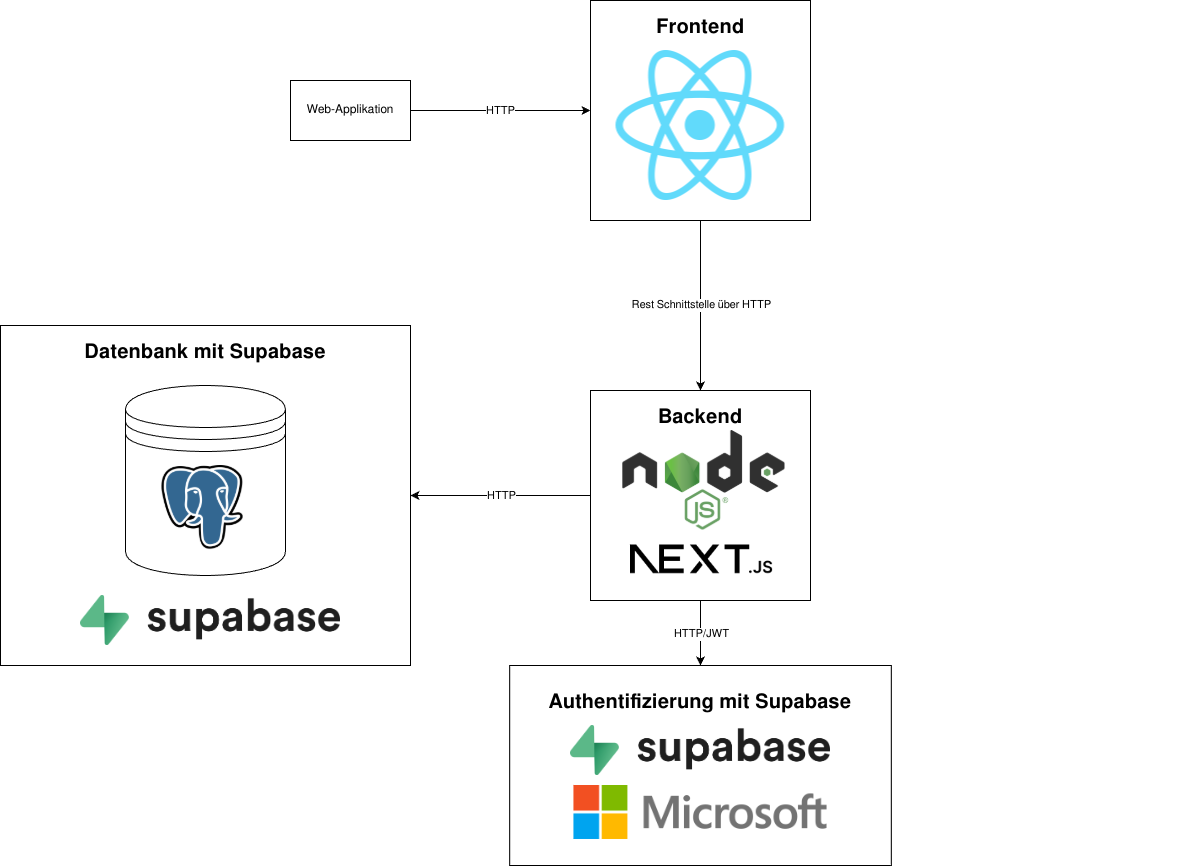
\includegraphics[width=0.8\textwidth]{Abbildungen/Systemarchitektur.png}
  \caption{Systemarchitektur}
  \label{fig:systemarchitektur}
\end{figure}

\newpage

%----------------------------------------------
% 7.2 Struktursicht
%----------------------------------------------

\subsection{Struktursicht}
\begin{figure}[H]
  \centering
  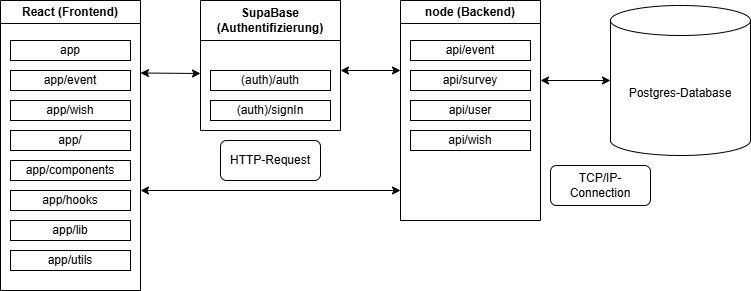
\includegraphics[width=1\textwidth]{Abbildungen/struktursicht.png}
  \caption{Struktursicht}
  \label{fig:struktursicht}
\end{figure}
Die Struktursicht zeigt den Aufbau des Projekts, das mit Next.js als Fullstack-Framework umgesetzt wurde. Die Anwendung ist in drei Hauptbereiche unterteilt: Das Frontend basiert auf React und ist modular strukturiert. Momentan wird für die Authentifizierung ein SSO benutzt, mit dem Authentication-Provider Google. Die Backend-Logik ist in Node.js implementiert und über die integrierten API-Routen von Next.js (z.B. api/event, api/user,...) realisiert. Es wird eine TCP/IP Verbindung für die Komunikation mit der Postgres-Datenbank genutzt. Die Architektur trennt somit klar zwischen Benutzeroberfläche, Geschäftslogik und Datenhaltung.

%----------------------------------------------
% 7.3 Verhaltenssicht
%----------------------------------------------

\subsection{Verhaltenssicht}
\begin{figure}[H]
  \centering
  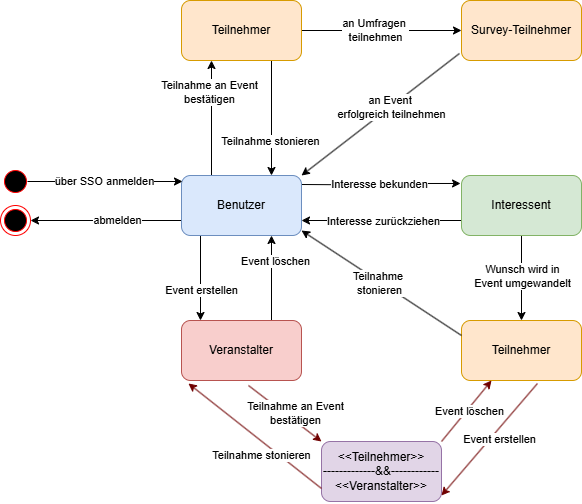
\includegraphics[width=0.9\textwidth]{Abbildungen/verhaltenssicht.png}
  \caption{Verhaltenssicht}
  \label{fig:verhaltenssicht}
\end{figure}
Die Verhaltenssicht beschreibt die Rollen und Interaktionen der Nutzer innerhalb der Anwendung. Ausgangspunkt ist der Benutzer, der sich über SSO anmelden und verschiedene Rollen einnehmen kann. Als Interessent kann er Interesse an einem Event bekunden oder zurückziehen. Sobald Interesse in eine Teilnahme übergeht, wird er zum Teilnehmer und kann Events bestätigen, stornieren oder an Umfragen teilnehmen. Wird ein Benutzer selbst aktiv, kann er als Veranstalter Events erstellen und verwalten. Die Grafik veranschaulicht diese dynamischen Zustandswechsel und Aktionen im System.

%----------------------------------------------
% 7.4 Verteilungssicht
%----------------------------------------------

\subsection{Verteilungssicht}
\begin{figure}[H]
  \centering
  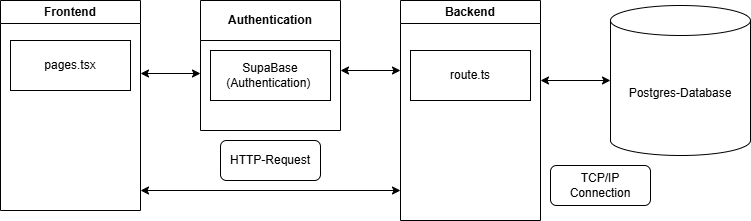
\includegraphics[width=1\textwidth]{Abbildungen/verteilungssicht.png}
  \caption{Verteilungssicht}
  \label{fig:verteilungssicht}
\end{figure}
Die Verteilungssicht zeigt, wie die verschiedenen Teile der Anwendung auf technische Komponenten verteilt sind. Das Frontend besteht aus React-Komponenten, die in pages.tsx implementiert sind. Die Authentifizierung erfolgt über SupaBase, das direkt vom Frontend per HTTP-Request angesprochen wird. Das Backend nutzt eine Datei wie route.ts, um serverseitige Logik bereitzustellen, und kommuniziert ebenfalls per HTTP mit der SupaBase-Datenbank. Die Datenhaltung sowie Authentifizierung sind somit ausgelagert und zentral über SupaBase realisiert. Die Struktur ermöglicht eine klare Trennung zwischen Präsentation, Authentifizierung, Logik und Daten.

\newpage

%----------------------------------------------
% 8. Schnittstellentechnologien
%----------------------------------------------

\section{Schnittstellentechnologien}

%----------------------------------------------
% 8.1 Technische Umsetzung der Schnittstelle
%----------------------------------------------

\subsection{Technische Umsetzung der Schnittstelle}
Schnitt\-stellen\-technologien bilden das Fundament für die reibungslose Kommunikation zwischen den verschiedenen Komponenten unseres Software\-systems. Ziel ist es, den Daten\-austausch zwischen Frontend, Backend und Authentifizierungs\-mechanismen klar zu strukturieren und zuverlässig zu gestalten. Für unser Projekt haben wir uns bewusst für eine \texttt{RESTful-API} entschieden, um eine klar strukturierte und standardisierte Schnittstelle bereitzustellen. Die zentrale Aufgabe unseres Systems besteht darin, Events und Event-Wünsche anzulegen, anzuzeigen, zu bearbeiten und zu löschen – typische Operationen also, die sich sehr gut durch das \texttt{\gls{CRUD}}-Modell (Create, Read, Update, Delete) abbilden lassen. \texttt{\gls{REST}} ist dabei nicht nur leicht verständlich, was die Entwicklung erleichtert, sondern hat auch die Zusammenarbeit im Team gefördert. Als Datenformat verwenden wir \texttt{JSON}, die Übertragung erfolgt über das \texttt{HTTPS}-Protokoll. Damit ist die Kommunikation platt\-form\-unabhängig, sicher und performant. Die Architektur der API orientiert sich am App-Router-Konzept von \mbox{\texttt{Next.js}}, wobei jede Route in einer eigenständigen Datei (z.\,B. \mbox{\texttt{app/api/.../route.ts}}) implementiert wird. Die Anbindung an die Datenbank erfolgt über \texttt{\gls{Prisma}}, die Benutzer\-verwaltung übernimmt \texttt{Supabase}. Ein weiterer Vorteil unserer \gls{API} ist die Zustands\-losigkeit: Jede Anfrage bringt alle nötigen Informationen mit, z.\,B. Auth-Daten per \texttt{\gls{JWT}}-Cookie. Dadurch brauchten wir keine eigene Session\-Verwaltung. Auch bei der \texttt{URI}-Struktur setzen wir auf klare Adressierbarkeit, so wie beim Abrufen aller Events über \mbox{\texttt{GET /api/Event}} oder dem Upvote via \mbox{\texttt{POST /api/wish/[wishId]/upvote}}. In der folgenden Tabelle \ref{tab:api-events} sind exemplarisch die wichtigsten Endpunkte für Events dargestellt:
\begin{table}[H]
\centering
\scriptsize
\begin{tabularx}{\textwidth}{|l|l|X|X|X|}
\hline
\textbf{Methode} & \textbf{Pfad} & \textbf{Beschreibung} & \textbf{Erfolgsstatus} & \textbf{Fehlerstatus} \\ \hline
GET    & \texttt{/api/event}         & Gibt eine Liste aller Events zurück                     & 200 OK                            & 500 Internal Server Error           \\ \hline
POST   & \texttt{/api/event}         & Erstellt ein neues Event                                & 201 Created                       & 400 Bad Request                     \\ \hline
GET    & \texttt{/api/event/[id]}    & Gibt ein einzelnes Event mit zugehörigen Daten zurück   & 200 OK                            & 500 Internal Server Error           \\ \hline
PATCH  & \texttt{/api/event/[id]}    & Aktualisiert gezielt Felder eines Events inkl. Terminen & 200 OK oder 201 Created           & 400 Bad Request, 404 Not Found      \\ \hline
DELETE & \texttt{/api/event/[id]}    & Löscht ein Event                                        & 200 OK oder 204 No Content        & 404 Not Found                       \\ \hline
\end{tabularx}
\caption{Exemplarische Endpunkte der Event-API}
\label{tab:api-events}
\end{table}

\noindent
PUT ist aktuell nicht implementiert, da im Projekt nur gezielte Änderungen nötig waren, ein vollständiges Überschreiben per PUT war bisher nicht erforderlich. Die verwendeten HTTP-Methoden entsprechen dem CRUD-Paradigma: Leseoperationen werden durch GET realisiert, das Anlegen neuer Ressourcen oder das Auslösen von Aktionen erfolgt mittels POST, während PATCH für gezielte Aktualisierungen und DELETE für das Entfernen von Ressourcen zuständig ist. Die aktuellen APIs sind im GitHub-Repository mittels einer OpenAPI-Swagger-Datei dokumentiert

\newpage

%----------------------------------------------
% 9. Datenbank
%----------------------------------------------

\section{Datenbank}

%----------------------------------------------
% 9.1 Logisches Datenmodell
%----------------------------------------------

\subsection{Logisches Datenmodell}

\begin{figure}[h]
  \centering
  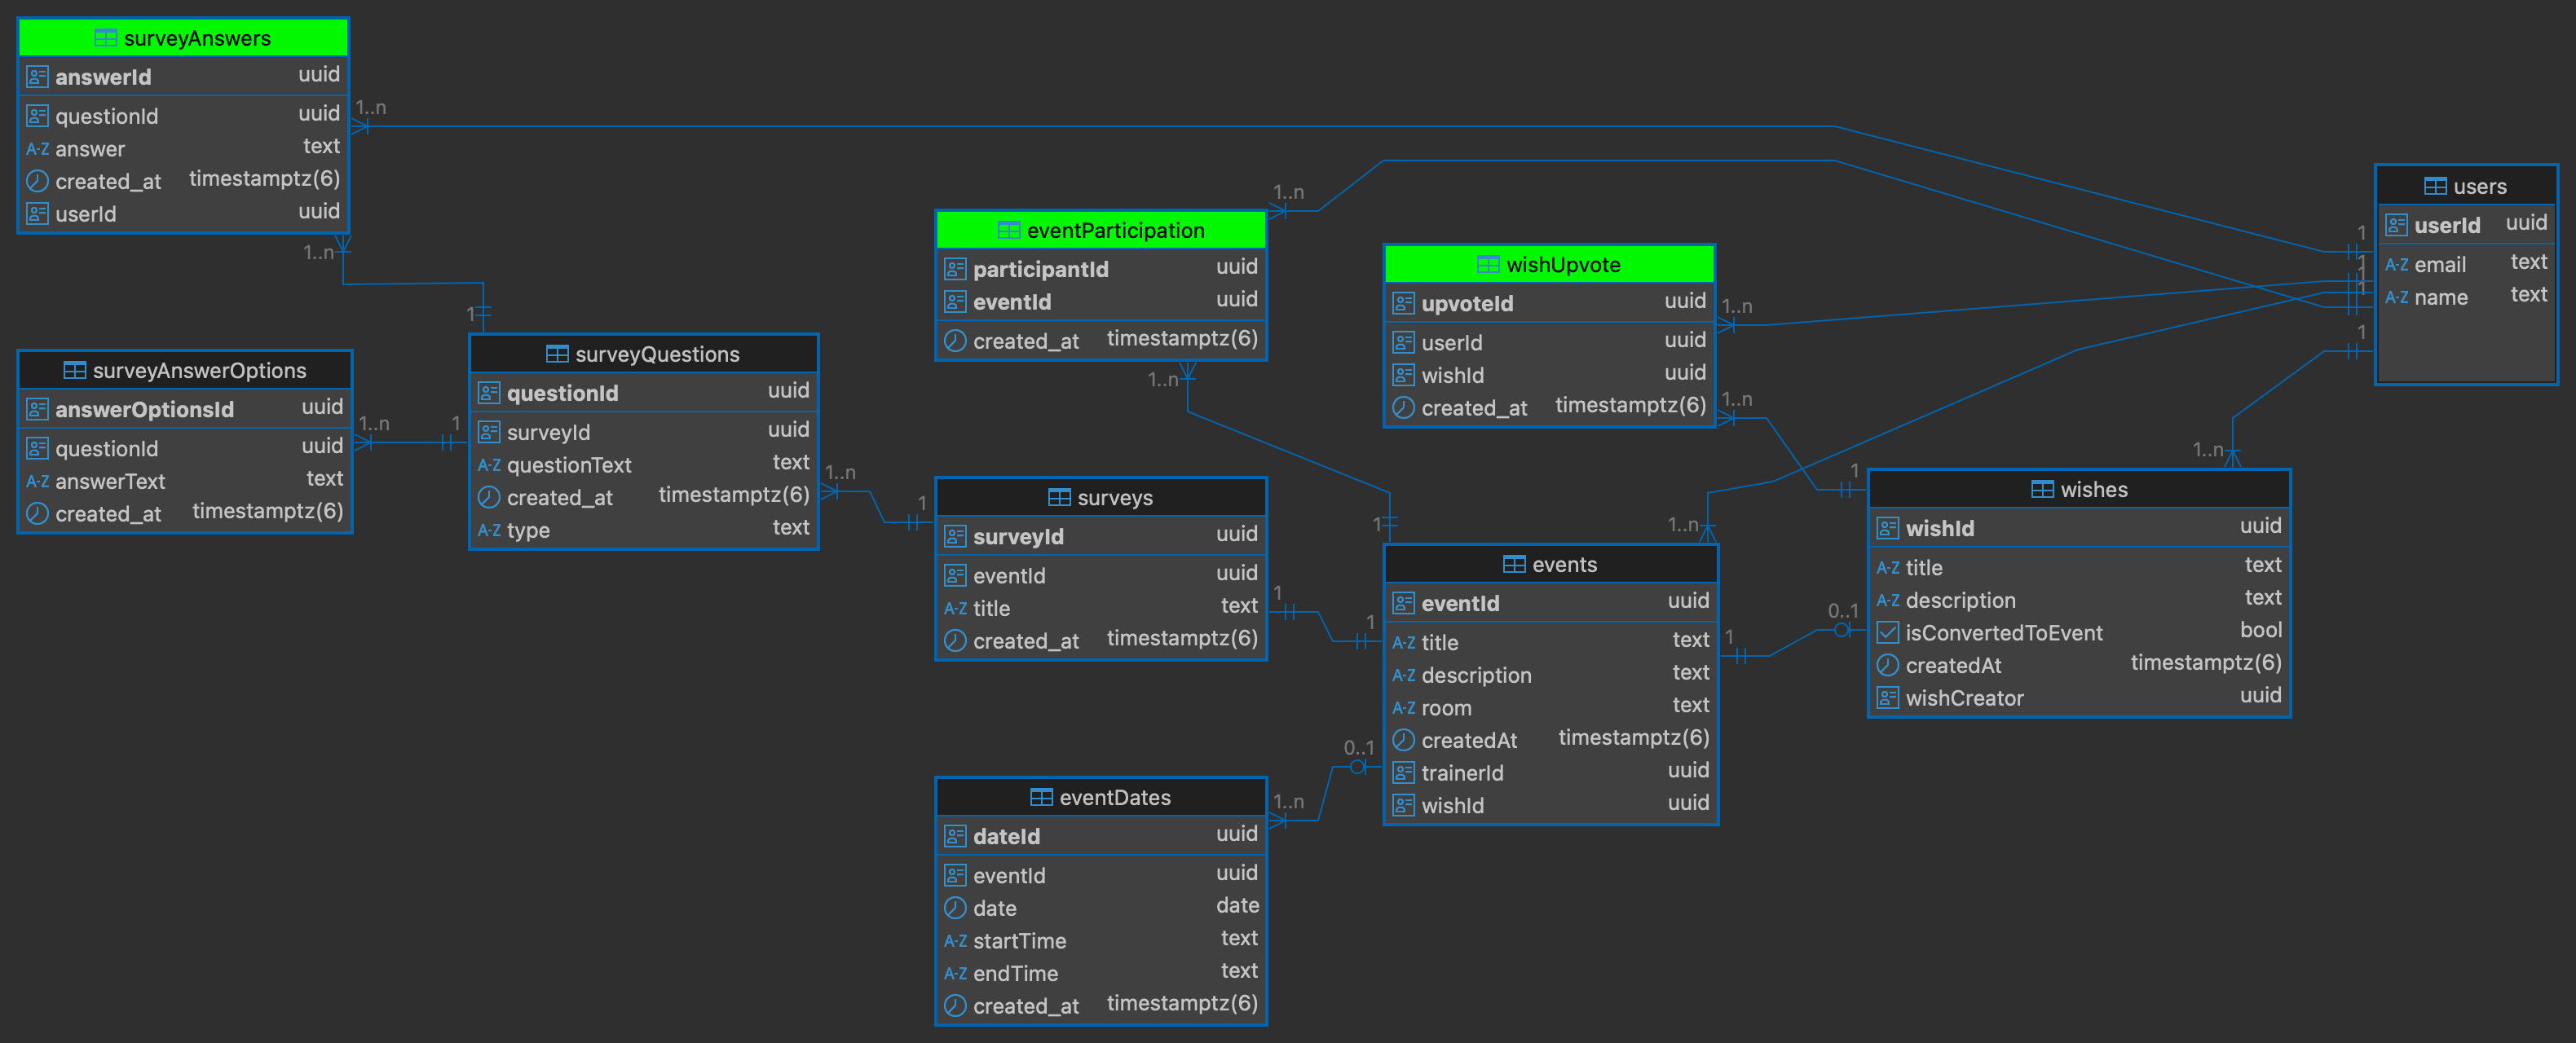
\includegraphics[width=1\textwidth]{Abbildungen/erm.png}
  \caption{Logisches Datenmodell}
  \label{fig:logisches_datenmodell}
\end{figure}

%----------------------------------------------
% 9.1.1 Entity Relationship Modell
%----------------------------------------------

\subsubsection{Entity Relationship Modell}
Die Anwendung verwendet eine relationale Datenbank auf Basis von PostgreSQL. Die Entscheidung fiel bewusst auf PostgreSQL, da es sich um ein bewährtes, leistungsstarkes Open-Source-Datenbanksystem handelt, das ACID-Konformität, flexible Abfragemöglichkeiten sowie gute Skalierbarkeit bietet – alles zentrale Anforderungen für das Eventmanagement, Umfrageverarbeitung und die Wunsch-Einreichung in der Anwendung. Zur Verwaltung und Bereitstellung der Datenbank wird Supabase verwendet, ein Backend-as-a-Service-Framework, das PostgreSQL als Kerntechnologie nutzt. Supabase bietet zusätzlich integrierte Funktionen wie Supabase Auth für die Authentifizierung, das in der Anwendung für die gesamte Authentifizierung und Nutzerverwaltung verwendet wird. Dadurch lässt sich der Entwicklungsaufwand im Backend deutlich reduzieren, ohne auf Sicherheit und Konsistenz bei der Zugriffskontrolle verzichten zu müssen.

%----------------------------------------------
% 9.1.2 Nutzerverwaltung
%----------------------------------------------

\subsubsection{Nutzerverwaltung}
Ein zentraler Bestandteil dieser Architektur ist die enge Verknüpfung zwischen der eigens entwickelten Users-Tabelle und der von Supabase bereitgestellten Tabelle auth.users. Während sicherheitskritische Informationen wie Passwörter ausschließlich in auth.users abgelegt und geschützt bleiben, enthält die eigene Users-Tabelle ergänzende Angaben wie E-Mail-Adresse oder Anzeigename. Die Verbindung beider Tabellen erfolgt über das id-Feld, das in auth.users als Primary Key definiert ist. Ein automatisch ausgelöster Trigger sorgt dafür, dass diese ID unmittelbar nach der Registrierung auch in der Users-Tabelle als Foreign Key gespeichert wird. Dadurch wird jeder Nutzer eindeutig identifizierbar und eine klare Trennung zwischen sicherheitsrelevanten und anwendungsbezogenen Informationen geschaffen.

%----------------------------------------------
% 9.1.3 Haupttabellen und ihre Aufgabenbereiche
%----------------------------------------------

\subsubsection{Haupttabellen und ihre Aufgabenbereiche}
Die Datenbankstruktur gliedert sich in Haupt- und Hilfstabellen (vgl. Abbildung \ref{fig:logisches_datenmodell}). Die Haupttabellen sind in der Abbildung schwarz dargestellt, während die Hilfstabellen farblich hervorgehoben (grün) sind. Zu den Haupttabellen zählen neben Users auch Wishes, Events sowie Surveys und SurveyQuestions. Über Wishes lassen sich Vorschläge - etwa für künftige Schulungsveranstaltungen - einreichen. Diese Vorschläge können von anderen Nutzern geupvoted oder in tatsächliche Events umgewandelt werden. Solche Events können jedoch auch unabhängig von Wünschen erstellt werden. Surveys ermöglichen es, Rückmeldungen einzuholen, beispielsweise zur Qualität von Events, und sind direkt mit den dazugehörigen SurveyQuestions verknüpft, die die konkreten Fragestellungen enthalten.

%----------------------------------------------
% 9.1.4 Hilfstabellen für komplexe Beziehungen
%----------------------------------------------

\subsubsection{Hilfstabellen für komplexe Beziehungen}
Die Hilfstabellen dienen vor allem der Abbildung komplexer, meist Viele-zu-Viele-Beziehungen. So wird in UserAnswer gespeichert, welche Antwort ein bestimmter Nutzer auf eine Umfragefrage gegeben hat. Die Tabelle EventParticipation dokumentiert, welche Nutzer sich für welche Events angemeldet haben. WishUpvote wiederum ermöglicht es, Schulungswünsche zu unterstützen, indem man signalisiert, dass man die Idee für sinnvoll hält und sich eine Umsetzung in Form eines Events wünscht.

%----------------------------------------------
% 9.2 Physisches Datenmodell
%----------------------------------------------

\subsection{Physisches Datenmodell}
Das zuvor beschriebene logische Datenmodell wurde in PostgreSQL vollständig umgesetzt. Dabei wurde insbesondere auf Datenintegrität, Normalisierung und den gezielten Einsatz eines Triggers zur Pflege der eigenen Users-Tabelle geachtet. Primärschlüssel werden durchgängig als uuid realisiert, um eine systemübergreifend eindeutige Identifikation von Datensätzen zu gewährleisten. Alle Beziehungen zwischen den Tabellen sind über Foreign-Key-Constraints abgesichert, sodass beispielsweise ein Nutzer nur dann an einem Event teilnehmen oder eine Umfrage beantworten kann, wenn er zuvor auch für das entsprechende Event registriert wurde. Die referenzielle Integrität wird durch entsprechende Foreign-Key-Constraints auf Datenbankebene gewährleistet. Die Datenbankstruktur wurde in der dritten Normalform (3NF) gehalten. Im Datenmodell ist dies erkennbar an der konsequenten Trennung von Entitäten wie Users, Wishes, Events und Surveys, die jeweils klar abgegrenzte Aufgabenbereiche und Attribute besitzen. Jede Tabelle enthält ausschließlich Attribute, die direkt vom Primärschlüssel abhängig sind. Es gibt keine transitive Abhängigkeit zwischen Nicht-Schlüsselattributen. Beispielsweise sind die Antworten auf Umfragen klar normalisiert: Die gewählten Optionen (SurveyAnswerOptions) und die tatsächlichen Nutzerantworten (SurveyAnswers) sind strikt getrennt, inklusive eindeutiger Referenzen auf Fragen und Nutzer. Durch diese Struktur wird Redundanz vermieden. Die Tabelle Users ist über das Feld userId mit der Supabase-Authentifizierungstabelle auth.users verknüpft. Wie in Abschnitt 9.1.2 beschrieben, stellt ein in PostgreSQL implementierter Trigger sicher, dass beim Anlegen eines neuen Auth-Users automatisch ein entsprechender Eintrag in der eigenen Users-Tabelle erzeugt wird. Dies gewährleistet eine saubere Trennung sicherheitsrelevanter Informationen von anwendungsspezifischen Profildaten.

\newpage

%----------------------------------------------
% 10. Installations- & Administrationshandbuch
%----------------------------------------------

\section{Installations- \& Administrationshandbuch}

Die Installations- und Administrationsanleitung befindet sich vollständig dokumentiert in der Datei README.md im Hauptverzeichnis des GitHub-Repositories. Darin werden zwei Varianten zur Ausführung der Anwendung beschrieben: eine lokale Installation sowie eine containerisierte Ausführung mittels Docker.

%----------------------------------------------
% 10.1 Lokale Installation
%----------------------------------------------

\subsection{Lokale Installation}

Für die lokale Nutzung werden Node.js (Version 18 oder höher), ein Paketmanager (npm oder yarn) sowie eine PostgreSQL Datenbank die bei diesem Projekt über Supabase läuft vorausgesetzt. Die notwendigen Umgebungsvariablen sind in einer .env-Datei zu definieren, für die eine Vorlage in der Datei .env.template bereitgestellt wird.

Die Schritte zur Installation und Ausführung beinhalten unter anderem:

\begin{itemize}
  \item Klonen des Repositories
  \item Installation der Abhängigkeiten
  \item Generierung des Prisma-Clients
  \item Start der Anwendung im Entwicklungs- oder Produktionsmodus
\end{itemize}

Zudem werden administrative Befehle für Prisma dokumentiert, etwa zur Migration oder zur Verwendung des webbasierten Datenbank-Interfaces.

%----------------------------------------------
% 10.2 Containerisierte Ausführung mit Docker
%----------------------------------------------

\subsection{Containerisierte Ausführung mit Docker}

Alternativ kann die Anwendung vollständig containerisiert ausgeführt werden. Die dazu erforderlichen Konfigurationsdateien Dockerfile und docker-compose.yml sind im Projekt enthalten. Die Docker-Umgebung berücksichtigt unter anderem die Abhängigkeit von OpenSSL und die Nutzung von Supabase mit einem IPv4-kompatiblen Session Pooler.

Die README-Datei beschreibt den Aufbau, Start, Betrieb und das Stoppen der Containerumgebung sowie die Ausführung von Verwaltungsbefehlen innerhalb des Containers.

%----------------------------------------------
% 10.3 Projektstruktur
%----------------------------------------------

\subsection{Projektstruktur}

Ebenfalls in der README.md enthalten ist ein Überblick über die Projektstruktur, einschließlich Konfigurationsdateien, Verzeichnisse für Quellcode, Datenbankschemata und Containerdefinitionen.

\vspace{1em}
\noindent\textit{Hinweis: Dem Dokument wurden die benötigten Umgebungsvariablen hinzugefügt, da diese für die Ausführung der Anwendung erforderlich sind.}

\newpage

%----------------------------------------------
% 11. Lizenzen 
%----------------------------------------------

\section{Lizenzen}

\subsection{Verwendete Lizenzen}

Im Projekt wird das Framework Next.js verwendet, das unter der MIT-Lizenz steht. Darüber hinaus kommen zahlreiche weitere Open-Source-Bibliotheken zum Einsatz, die überwiegend ebenfalls unter der MIT-Lizenz veröffentlicht wurden. Dazu gehören unter anderem:

\begin{itemize}
  \item React und React-DOM (MIT)
  \item Prisma (MIT)
  \item MUI (Material UI) (MIT)
  \item Emotion (verschiedene Module wie styled, cache, react) (MIT)
  \item Axios (MIT)
  \item Date-fns und date-fns-tz (MIT)
  \item Supabase (MIT)
  \item EJS (Apache-2.0)
  \item Diverse ESLint- und Testing-Bibliotheken (überwiegend MIT)
\end{itemize}

Die genauen Lizenzinformationen aller verwendeten Pakete sind in der Datei package-lock.json hinterlegt. Dabei handelt es sich fast ausschließlich um weit verbreitete, permissive Lizenzen wie MIT, Apache-2.0 oder BSD.

\subsection{Lizenz des eigenen Quellcodes}

Der im Rahmen dieses Projekts erstellte Quellcode wird unter die MIT-Lizenz gestellt. Die Lizenz erlaubt eine freie Nutzung, Veränderung und Weiterverbreitung des Codes, auch für kommerzielle Zwecke, sofern die Lizenzbedingungen eingehalten werden. Der vollständige Lizenztext befindet sich in der Datei \texttt{LICENSE} im Hauptverzeichnis des Projekts.


\newpage

%----------------------------------------------
% 12. Ausblick
%----------------------------------------------

\section{Ausblick}

Das bisherige Event-Planer erfüllt alle gewünschten Anforderungen und funktioniert im Alltag zuverlässig. Trotzdem ergeben sich beim Arbeiten mit der Anwendung viele Ideen, wie sie in Zukunft weiterentwickelt werden könnte

%----------------------------------------------
% 12.1 Kalenderansicht / Kalendersystem
%----------------------------------------------

\subsection{Kalenderansicht / Kalendersystem}

Momentan werden geplante Events in einer einfachen Feed-Liste angezeigt. Für viele Nutzer könnte es hilfreicher sein, diese Veranstaltungen zusätzlich in einem Kalender zu sehen. Eine klassische Monats- oder Wochenansicht kann einen besseren Überblick über anstehende Termine vermittelt. Durch einen solchen Kalender würde erkennbar, wie stark bestimmte Tage belegt sind oder wo noch Platz für weitere Veranstaltungen bleibt. Auch Terminüberschneidungen oder Lücken im Plan würden sichtbar. Gerade wenn mehrere Events organisiert oder besucht werden, könnte diese visuelle Darstellung dabei helfen, schneller Entscheidungen zu treffen. Für den kann Kunden kann so ein Mehrwert entstehen, denn die Anwendung wirkt strukturierter und lässt sich flexibler im Alltag einsetzen.

\begin{figure}[H]
    \centering
    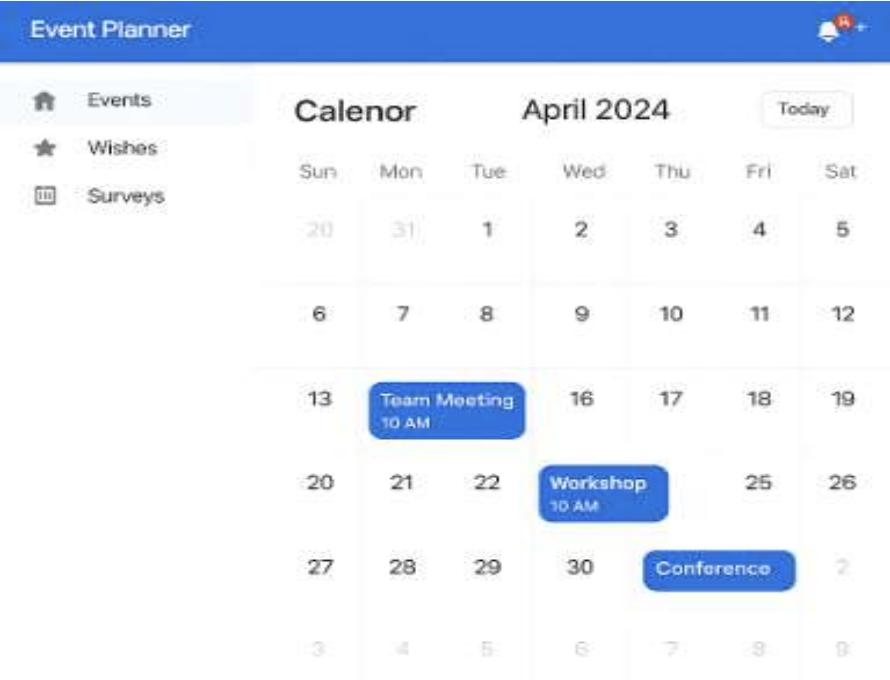
\includegraphics[width=1\textwidth]{Abbildungen/kalenderansicht.png}
    \caption{Kalendersystem (KI-generiert mit ChatGPT-4o, OpenAI, 2025)}
    \label{fig:kalenderansicht}
\end{figure}

\newpage

%----------------------------------------------
% 12.2 Zeitlich gruppierter Eventseite
%----------------------------------------------

\subsection{Zeitlich gruppierter Eventseite}

Aktuell werden die Events einfach untereinander angezeigt, egal ob sie heute stattfinden oder erst in ein paar Wochen. Das ist zwar funktional, aber mit der Zeit wird es unübersichtlich. Eine Gruppierung nach Zeitabschnitten könnte helfen.

\textbf{Die Idee}: Events werden automatisch nach ihrem Startdatum sortiert und in logische Abschnitte gegliedert, zum Beispiel \textbf{„Heute“}, \textbf{„Diese Woche“}, \textbf{„Nächste Woche“} oder auch einfach mit einem Datumstitel. So erkennt man auf einen Blick, was demnächst ansteht, ohne einzeln in der EventDetail-Seite suchen zu müssen. Das könnte praktisch für Vielnutzer oder bei größeren Organisationen mit zahlreichen Events werden.

\begin{figure}[H]
    \centering
    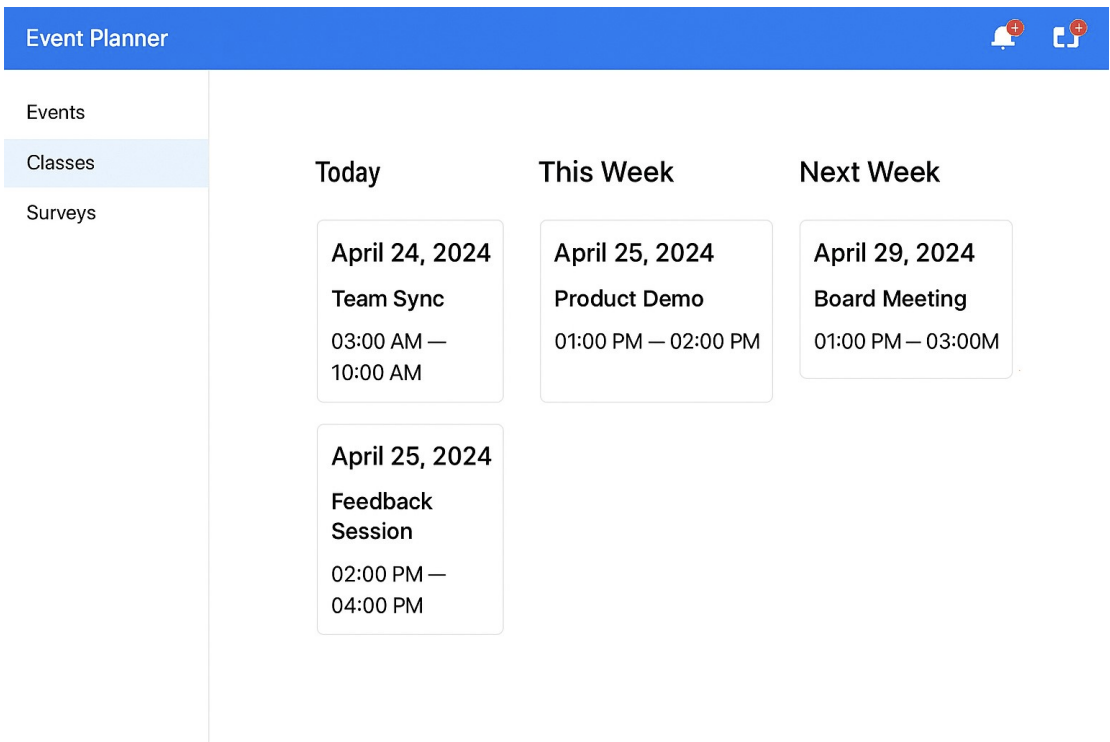
\includegraphics[width=1\textwidth]{Abbildungen/gruppierte_events.png}
    \caption{Events gruppiert nach Zeitabschnitten (generiert mit ChatGPT-4o, OpenAI, 2025)}
    \label{fig:gruppierte_events}
\end{figure}

\newpage

%----------------------------------------------
% 12.3 Kommentarsektion
%----------------------------------------------

\subsection{Kommentarsektion}

Obwohl alle grundlegenden Informationen zu einem Event direkt auf der Detailseite ersichtlich sind und sogar eigene Umfragen erstellt werden können, fehlt bisher eine einfache Möglichkeit, sich spontan oder informell auszutauschen.

Ein Kommentarbereich würde genau hier ansetzen. Teilnehmer könnten sich dort kurzschließen, wenn jemand etwas mitbringen möchte. Auch organisatorische Hinweise, die nicht direkt in die Eventbeschreibung gehören, hätten dort ihren Platz

So entsteht Raum für lockere Kommunikation direkt am Ort. Das könnte die Plattform persönlicher und interaktiver machen.

\begin{figure}[H]
    \centering
    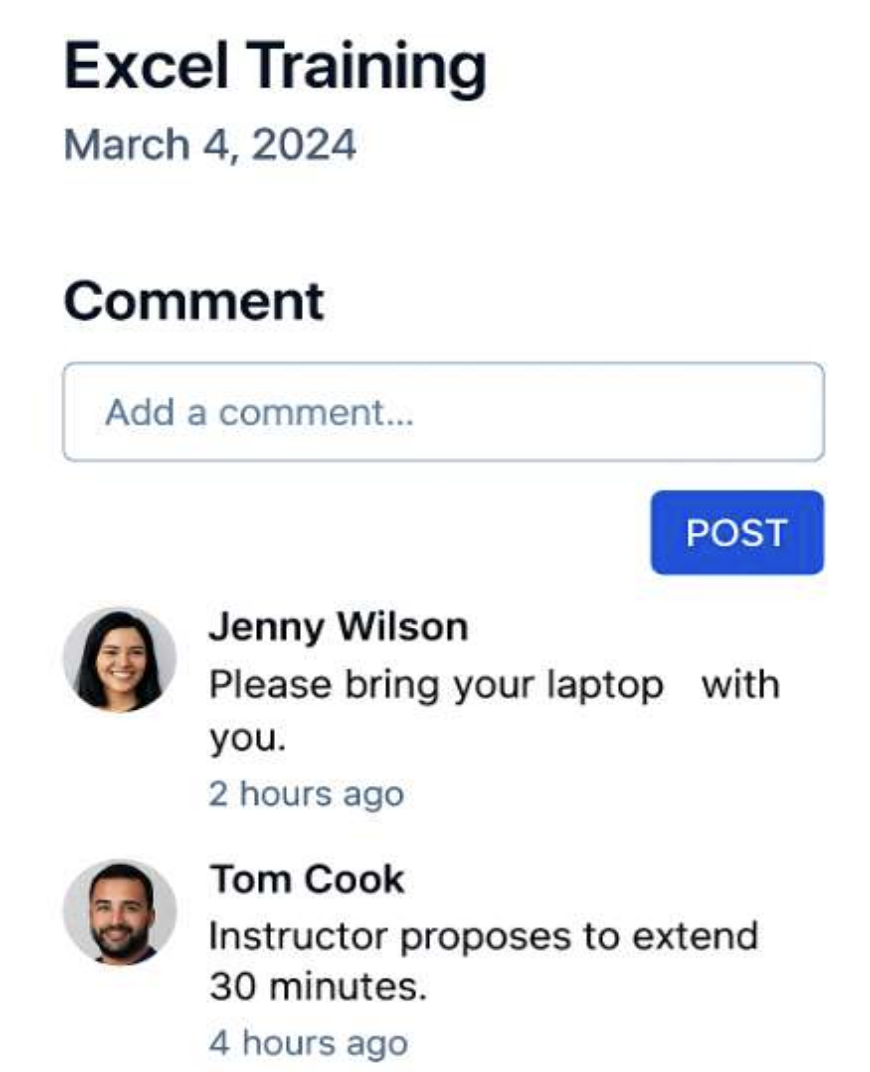
\includegraphics[width=0.7\textwidth]{Abbildungen/kommentarsektion.png}
    \caption{Kommentarsektion (generiert mit ChatGPT-4o, OpenAI, 2025)}
    \label{fig:kommentarsektion}
\end{figure}

\newpage

%----------------------------------------------
% 12.4 Profilseite
%----------------------------------------------

\subsection{Profilseite}

Aktuell gibt es in der Anwendung keine Möglichkeit, das eigene Profil einzusehen oder zu bearbeiten. Wer eingeloggt ist, sieht weder die eigene Mailadresse noch frühere Aktivitäten oder Events, an denen man teilnimmt. Auch andere Nutzerprofile sind nicht erreichbar.

Eine persönliche Profilseite würde genau hier ansetzen. Nutzer könnten dort ihre bisherigen Events einsehen, z. B. als Teilnehmer oder Organisator. Auch grundlegende Profilinformationen wie Name, E-Mail oder ein Avatar ließen sich dort darstellen und eventuell bearbeiten.

Das könnte nicht nur die Nutzerbindung verbessern, sondern auch Orientierung schaffen, wer hinter welchen Events oder Ideen steckt.

\begin{figure}[H]
    \centering
    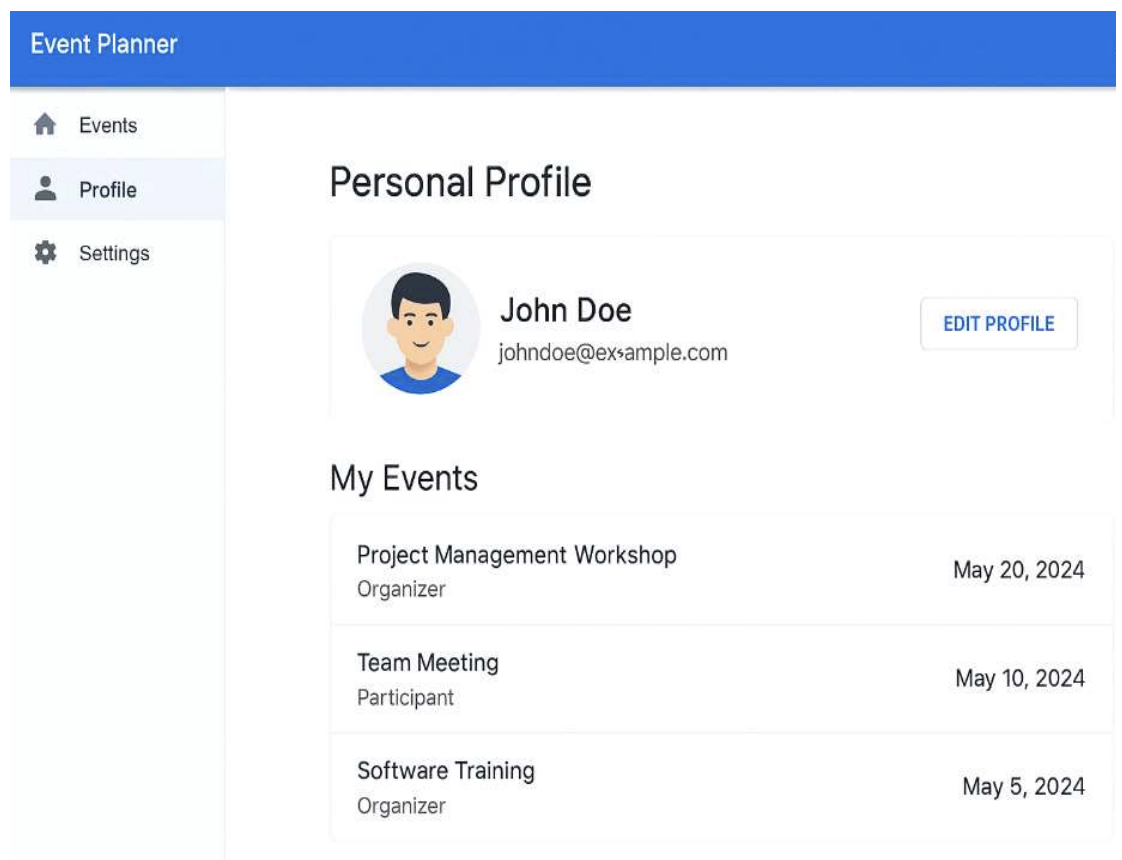
\includegraphics[width=1\textwidth]{Abbildungen/profilseite.png}
    \caption{Profilseite (generiert mit ChatGPT-4o, OpenAI, 2025)}
    \label{fig:profilseite}
\end{figure}

\newpage

%----------------------------------------------
% 12.5 Wiederkehrende Events
%----------------------------------------------

\subsection{Wiederkehrende Events}

Im System gibt es viele wiederkehrende Formate wie interne Schulungen oder Vorträge. Momentan müssen sie jedes Mal neu erstellt werden, auch wenn sich nur das Datum ändert. Es könnte den Komfort verbessern, wenn man beim Anlegen eines Events direkt angeben könnte, dass es sich wiederholt. Ob wöchentlich, monatlich oder nach einem benutzerdefinierten Rhythmus. Das System würde dann automatisch eine Event-Serie anlegen. Die Inhalte bleiben dabei gleich, nur die Termine unterscheiden sich. Gerade bei Formaten wie internen Schulungen spart das viel Aufwand und sorgt dafür, dass keine Termine vergessen werden. Auch für Teilnehmende kann es transparenter werden, wann die nächsten Sessions stattfinden.

\begin{figure}[H]
    \centering
    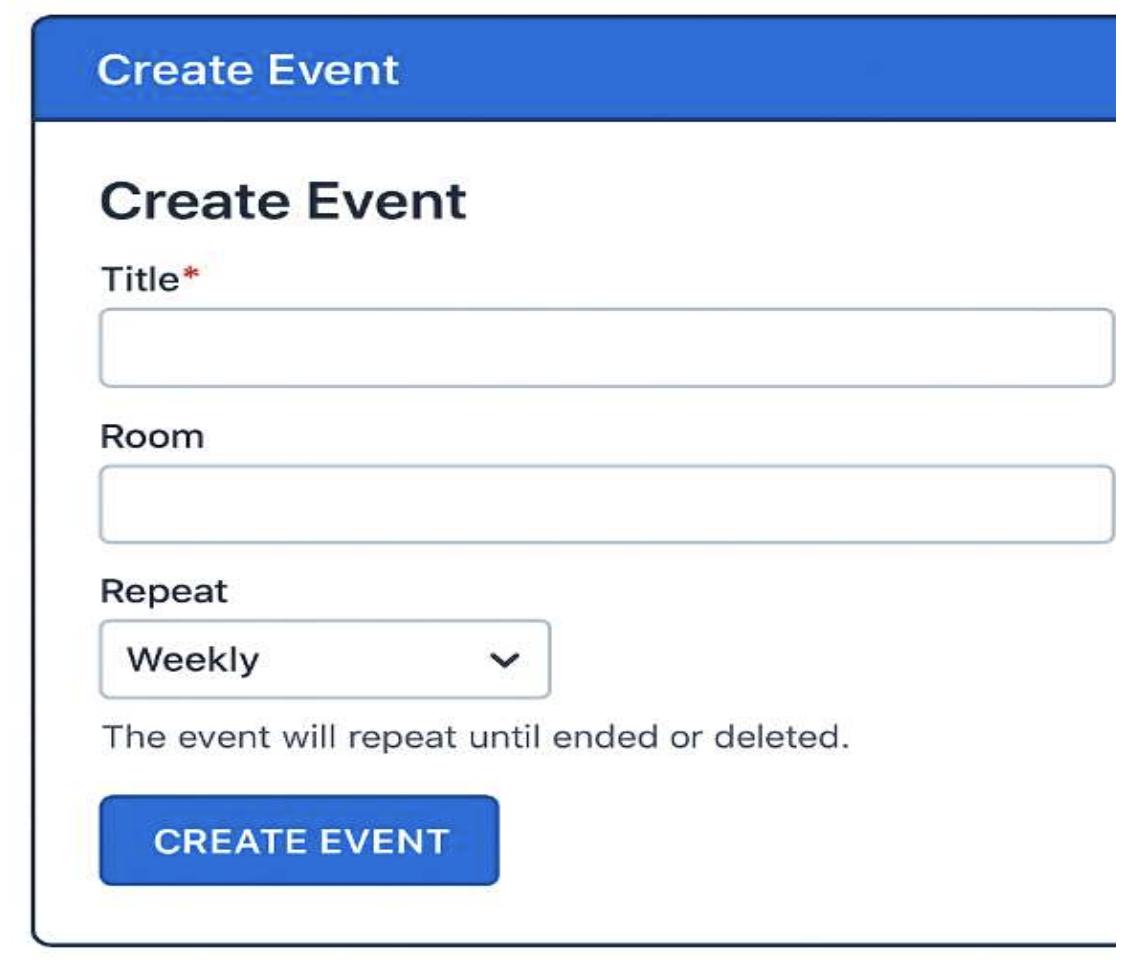
\includegraphics[width=1\textwidth]{Abbildungen/wiederkehrende_events.png}
    \caption{Wiederkehrende Events (generiert mit ChatGPT-4o, OpenAI, 2025)}
    \label{fig:wiederkehrende_events}
\end{figure}

\newpage

%----------------------------------------------
% 13. Aufgabenverteilung & Zusammenarbeit im Projekt
%----------------------------------------------

\section{Aufgabenverteilung \& Zusammenarbeit im Projekt}

Im Team Event-Planer hat grundsätzlich jede Person sowohl Frontend- als auch Backend-Aufgaben übernommen. Trotzdem haben sich im Laufe des Projekts natürliche Schwerpunkte gebildet, bei denen einzelne Mitglieder bestimmte Features federführend umgesetzt haben. 

Ergün war technischer Ansprechpartner, insbesondere im Bereich Authentifizierung und Supabase. Er hat die Anmeldung und Registrierung umgesetzt und dafür gesorgt, dass die Datenbank angebunden war. Außerdem hat er das \gls{Deployment} über \gls{Vercel} übernommen und sich um technische Aspekte gekümmert, die beispielsweise mit der Anbindung an die Cloud zusammenhingen. Zu Beginn des Projekts kam es aufgrund der Server-Region von Supabase, die zunächst in den USA lag, zu Latenzproblemen. Ergün hat in diesem Zusammenhang die Umstellung auf einen Server-Standort in Frankfurt organisiert. Zusätzlich hat er das Survey-Feature umgesetzt, das im Backend zusätzliche Logik erforderte. Auch bei Git-Problemen oder MergeKonflikten hat er häufig die Lösung übernommen.

Felix hat sich mit der E-Mail-Funktion beschäftigt, also mit allen Aspekten, die dafür sorgen, dass Teilnehmende bei bestimmten Aktionen automatisch benachrichtigt werden. Die Umsetzung erforderte eine enge Abstimmung zwischen Backend und Frontend. Darüber hinaus hat er beim \gls{Refactoring} mitgewirkt, den Code besser strukturiert und auf Übersichtlichkeit geachtet. 

Baran war vor bei der Datenbank und der Logik für Event-Teilnahmen aktiv. Er hat zu Beginn die Datenbank modelliert und diese anschließend fortlaufend an die Anforderungen angepasst. Zusätzlich hat er mit \gls{Balsamiq} eine erste visuelle Version der App erstellt, die in der weiteren Entwicklung genutzt wurde. Außerdem hat er Backend-Logik rund um Event-Teilnahmen sowie zusammen mit Sami das Statistik Feature umgesetzt.

Sami hat sich mit dem \gls{Upvote-Feature} beschäftigt, mit dem Nutzer Wishes bewerten können. Außerdem hat er die Logik für \gls{In-App-Benachrichtigungen} umgesetzt, also der Logik dahinter, wann Nutzer welche Informationen bekommen sollen, sowie der dazugehörigen Funktionalität. Ein weiterer Schwerpunkt war auch das Statistik Feature, bei dem er eng mit Baran zusammengearbeitet hat. Zusätzlich hat Sami das grundlegende Layout der App erstellt, einschließlich Navigation, Header und Footer, wodurch eine Struktur für die weitere Entwicklung entstand. Die Zusammenarbeit im Team verlief insgesamt strukturiert, auch wenn es Phasen gab, in denen einzelne Mitglieder überwiegend an spezifischen Features gearbeitet haben, wurden bei Problemen oder größeren Herausforderungen gemeinsame Lösungen erarbeitet. Die Arbeitsverteilung war ausgewogen, und alle Teammitglieder haben im Verlauf des Projekts sowohl im Backend als auch im Frontend Erfahrungen gesammelt.

\begin{figure}[H]
    \centering
    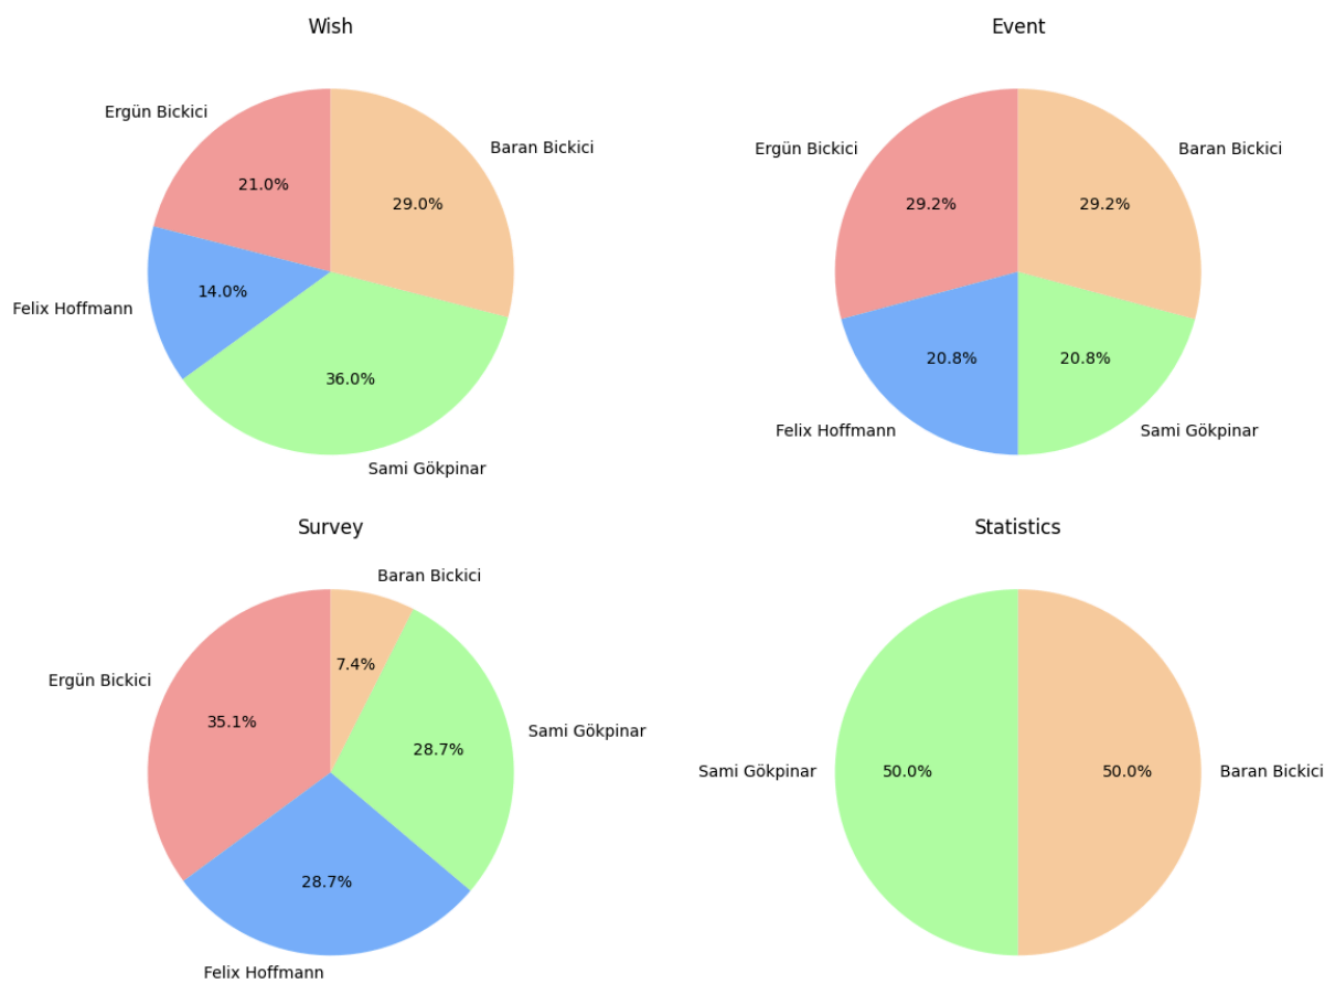
\includegraphics[width=1\textwidth]{Abbildungen/aufgaben_verteilung.png}
    \caption{Prozentuale Verteilung der Jira-Tickets nach Hauptfeature}
    \label{fig:aufgaben_verteilung}
\end{figure}

\noindent
Die Grafik zeigt die prozentualen Beiträge der einzelnen Teammitglieder zu den jeweiligen Hauptfeatures, basierend auf den erfassten Jira-Tickets. Dabei ist wichtig zu beachten, dass die dargestellten Prozentwerte den Anteil an der Gesamtarbeit innerhalb eines spezifischen Features widerspiegeln, nicht jedoch den Umfang oder Schwierigkeitsgrad der jeweiligen Funktion selbst 

Nicht alle Features sind gleich umfangreich oder komplex. Manche Bereiche, wie zum Beispiel das Statisticsoder Survey-Feature, bringen zusätzlichen technischen Aufwand mit sich, während andere eher frontendlastig sind oder sich stärker auf Design und Struktur konzentrieren. Die reine Aufteilung nach Ticket-Anteilen liefert daher nur einen groben Überblick, wer sich inhaltlich bei welchem Bereich eingebracht hat. Sie lässt jedoch keine direkten Rückschlüsse auf den tatsächlichen Zeit- oder Arbeitsaufwand zu. 

Die Visualisierung verdeutlicht dennoch die im Projekt entstandenen Schwerpunkte und bestätigt, dass einzelne Teammitglieder bestimmte Features federführend umgesetzt haben. Gleichzeitig zeigt sich auch, dass es übergreifende Zusammenarbeit gab, bei der alle Mitglieder in verschiedenen Bereichen mitgewirkt und sowohl Backend- als auch Frontend-Erfahrungen gesammelt haben.

\newpage

%----------------------------------------------
% 14. Vergleich von Aufwandsschätzung & Realaufwand
%----------------------------------------------

\section{Vergleich von Aufwandsschätzung \& Realaufwand}

Im Kurs wird von einer ungefähren wöchentlichen Arbeitszeit von 16 Stunden ausgegangen.
Zu Beginn des Projekts wurde der Zeitaufwand für die Planung der einzelnen Sprints unterschätzt. Das Erstellen vollständiger und für alle Entwickler verständlicher User-Stories benötigte regelmäßig bis zu zwei Stunden. Auch die Besprechungen mussten im Schnitt mit bis zu zwei Stunden bemessen werden. So nahmen die Sprintplanung und durchführung, unserer abstrahierten Version von Scrum, insgesamt bis zu fünf Stunden der wöchentlich angesetzten Arbeitszeit ein.

Unabhängig von der wöchentlichen Arbeitszeit hat das Erstellen einer stabilen Datenbankstruktur für den Event-Planer länger gedauert als ursprünglich erwartet. Die Planung der Datenbankstruktur nahm zu Beginn des Projekts neben dem Erstellen des Designs der Applikation einen großen Teil der Arbeitszeit ein. Die gesamte Zeit belief sich wie geschätzt auf knapp zwei Wochen. Jedoch wurden auch im Laufe des Projekts immer wieder Änderungen an der Datenbank vorgenommen, da unnötige Relationen oder Entitäten entfernt oder benötigte hinzugefügt wurden.

Dadurch zog sich die Entwicklung der Datenbank über nahezu das gesamte Projekt hinweg. Die Implementierung, also Umsetzung der einzelnen User-Stories, wurde von Beginn an als am zeitintensivsten eingeschätzt. Ein Großteil des Projektzeitraums (10 Wochen) wurde dafür und für die Tests eingeplant. Im Verlauf des Projekts stellte sich jedoch heraus, dass der tatsächliche Aufwand stark vom jeweiligen Thema abhing. Manche Aufgaben erwiesen sich wie erwartet als komplex, während andere deutlich einfacher umzusetzen waren. Oft, weil wir passende Technologien fanden, die uns einen Extraaufwand sparten. Beispielsweise konnte durch Prisma viel Zeit beim Erstellen und Ergänzen der Datenbankstruktur eingespart werden. Dabei kristallisierte sich heraus, dass das Einschätzen der Komplexität von Aufgaben eine Herausforderung ist. Die Einschätzungen fielen sehr unterschiedlich aus, typabhängig, mal eher vorsichtig, mal eher knapp Wöchentlich nahm die Bearbeitungszeit neben den organisatorischen Tätigkeiten rund um die Meetings den Rest der Woche ein, also mindestens 11 Stunden.

Die Dokumentation der gesamten Anwendung wurde bereits zu Beginn als aufwändig eingeschätzt, zum Beispiel das Dokumentieren der API-Schnittstellen. Im Verlauf des Projekts konnten wir jedoch durch die konsequente Nutzung von Jira, insbesondere durch das regelmäßige Erstellen von User-Stories und deren detaillierte Beschreibung, den dokumentarischen Aufwand besser bewältigen. Da User-Stories konsequent ausführlich ausformuliert und dokumentiert wurden, konnte auf diese Weise langfristig Zeit eingespart werden. Dennoch wurde auch der Aufwand für die Dokumentation der einzelnen Meilensteine als nicht unerheblich betrachtet. In der Woche vor den jeweiligen Abgaben ein Extra von drei Stunden.

Schlussendlich wurde der Aufwand für das Testen mit \gls{Unit-Tests} am stärksten unterschätzt. Durch die Ambition, am Ende eines jeden Sprints neue Features präsentieren zu können, war es nicht möglich, diese Features durch Unit-Tests zu prüfen. So wurde meistens manuell im Frontend getestet. Diese Arbeit summierte sich über den gesamten Projektverlauf hinweg und wurde schließlich so umfangreich, dass sie erst kurz vor der Projektabgabe abgeschlossen werden konnte.

\newpage

Das Projekt hat deutlich gemacht, wie essenziell Unit-Tests und Tests im Allgemeinen für die Stabilität einer Anwendung sind. Idealerweise sollten Tests vor oder spätestens während der Entwicklung neuer Features erstellt werden. In Abhängigkeit vom gewählten Entwicklungsansatz kann es sogar sinnvoll sein, Tests bereits vor Beginn der eigentlichen Implementierung zu formulieren. Auf diese Weise lassen sich viele Fehlerquellen frühzeitig erkennen und vermeiden. Auch die Belastung während der Entwicklungsphasen hätte durch eine frühzeitige Testabdeckung spürbar reduziert werden können. Zudem wurde deutlich, dass die Planung einzelner Sprints einen erheblichen Zeitaufwand darstellt.

Vor diesem Hintergrund lässt sich sagen, dass in Anbetracht der Zeit und des Umfangs für dieses Projekt ein linearer Ansatz, möglicherweise mit dem Ausformulieren eines Lastenhefts, effektiver gewesen wäre. Da so viel Organisationszeit für das Scrum verfahren gespart worden wäre. Da sich der Umfang des Projekts noch im unteren Teil am Ursprung der Stacey-Matrix einschätzen lässt.

Trotzdem war es richtig und gut, eine abgeänderte Form von Scrum als Projektorganisationsmethode zu nutzen, da Scrum ein weit verbreiteter Industriestandard ist und so wertvolle Einblicke in das Berufsleben gewonnen werden konnten.

\begin{figure}[H]
    \centering
    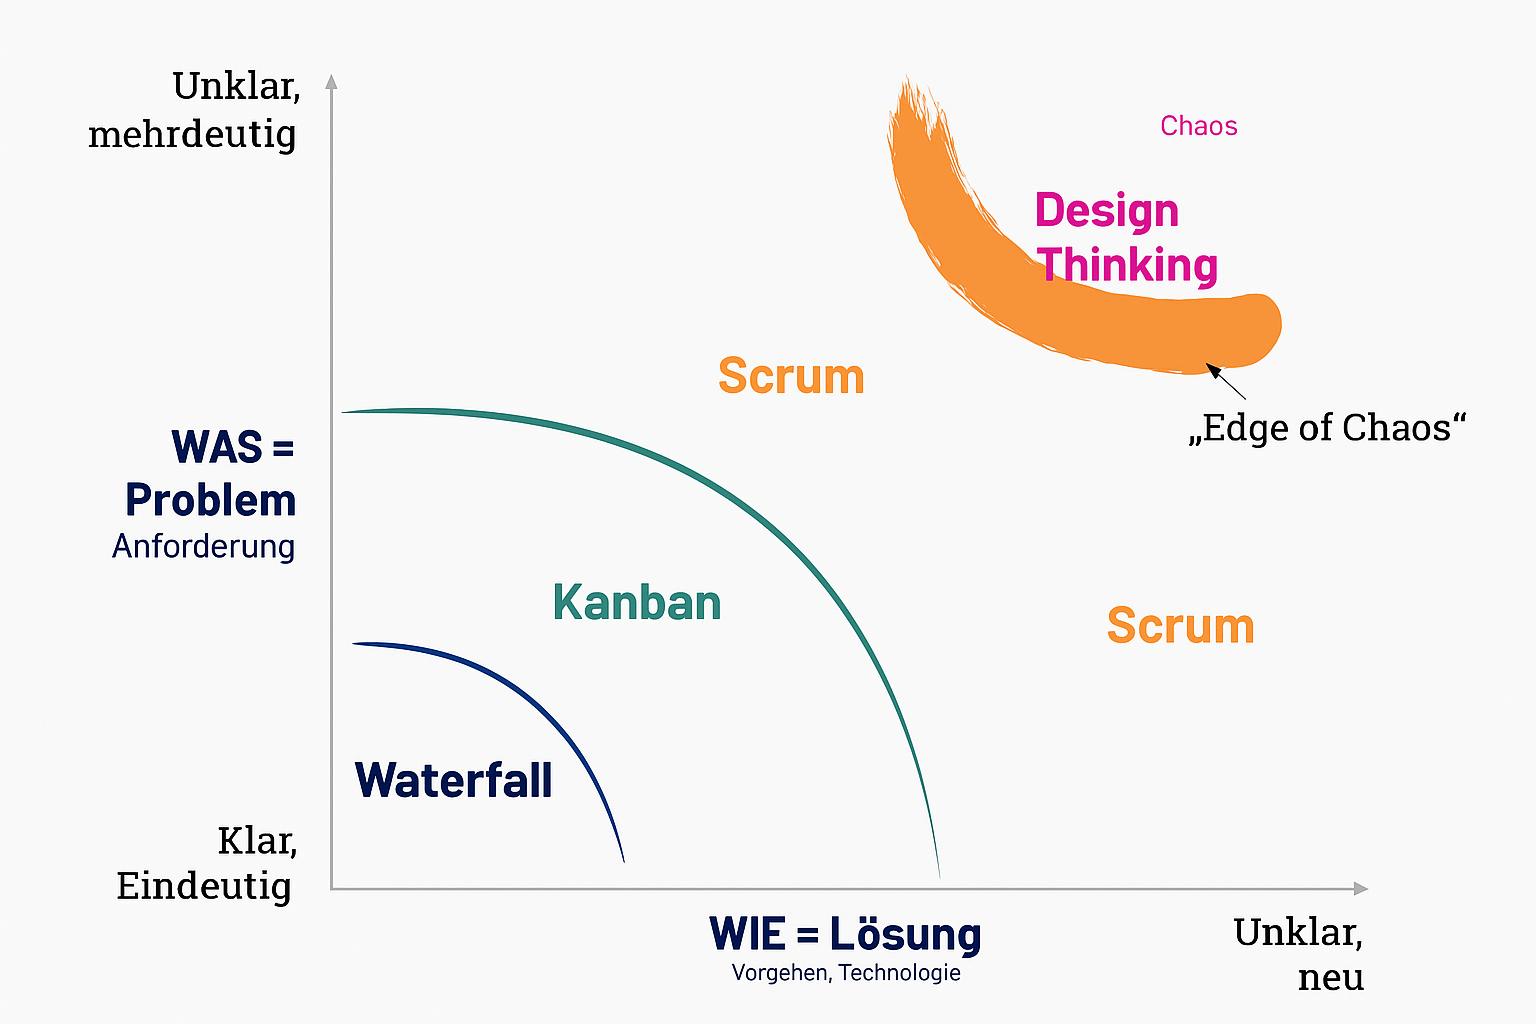
\includegraphics[width=1\textwidth]{Abbildungen/stacey_matrix.png}
    \caption{Stacey Matrix}
    \label{fig:stacey_matrix}
    \vspace{1mm}
    {\small Quelle: \url{https://chatgpt.com/s/m_6859cf49fe1c8191b4c5b9ef57609591}}
\end{figure}


\newpage

%----------------------------------------------
% 15. Reflexion & Lernfortschritt
%----------------------------------------------

\section{Reflexion \& Lernfortschritt}

Durch das Semesterprojekt, bei dem für ein reales Unternehmen eine praxisnahe Anwendung entwickelt wurde, konnten sowohl fachliche als auch persönliche Erfahrungen gesammelt werden. Im Verlauf des Semesters fanden regelmäßige Meetings mit dem Betreuer und dem Kunden statt, die dabei halfen, die Arbeit an den Anforderungen auszurichten und kontinuierlich weiterzuentwickeln.

%----------------------------------------------
% 15.1 Technische Fähigkeiten
%----------------------------------------------

\subsection{Technische Fähigkeiten}

Im technischen Bereich wurden umfangreiche neue Kenntnisse erworben. Technologien wie Next.js, Supabase und Prisma waren zu Beginn für die meisten Teammitglieder neu. Einzelne Personen verfügten bereits über erste Vorkenntnisse im Umgang mit Next.js. Dennoch war es erforderlich, sich intensiv mit diesen Tools auseinanderzusetzen und verschiedene Herausforderungen zu bewältigen. Im weiteren Verlauf des Projekts wurde der Umgang mit den Technologien vertrauter wodurch Funktionen wie Authentifizierung, automatisierte E-Mail-Benachrichtigungen und Datenbankmodellierungen umgesetzt werden konnten. Das Deployment über Vercel ermöglichte zudem praktische Einblicke in HostingPlattformen und produktive Umgebungen.

Ein zusätzlicher technischer Schwerpunkt lag im Umgang mit Git. Insbesondere zu Beginn traten häufig \gls{Merge-Konflikte} auf. Trotz der Nutzung von \gls{Feature-Branches} kam es zu Überschneidungen, die im Technische Fähigkeiten Vorfeld nicht immer absehbar waren. Teilweise arbeiteten mehrere Personen parallel an denselben Komponenten, was die Konflikte begünstigte. Um diese Probleme zu reduzieren, wurde der Fokus stärker auf technisches Planen und Abstimmung innerhalb des Teams gelegt. Die Anwendung systematischer Fehleranalysen unterstützte dabei den Entwicklungsprozess. Insbesondere durch \gls{Debugging} konnten Fehler schrittweise erkannt und behoben werden.

Im Bereich Testing und Qualitätssicherung wurde erkannt, wie wichtig automatisierte Tests für die langfristige Stabilität sind. Während der Projektphase wurden überwiegend manuelle Tests durchgeführt, indem die Anwendung wiederholt durchgeklickt und Funktionen überprüft wurden. Dennoch traten weiterhin Fehler auf, die teilweise vom Betreuer oder dem Kunden entdeckt wurden. Im Rückblick zeigte sich, dass ein früherer und konsequenter Einsatz von automatisierten Tests, einschließlich \gls{Exploratory-Tests} Unit-Tests und \gls{End-to-End-Tests}, dabei geholfen hätte, solche Fehler frühzeitig zu identifizieren.

%----------------------------------------------
% 15.2 Methodische Kompetenzen
%----------------------------------------------

\subsection{Methodische Kompetenzen}

Neben den technischen Aspekten lag der Fokus zunehmend darauf, das Projekt strukturiert und wartbar umzusetzen. Regelmäßige RefactoringProzesse und Code Reviews unterstützten dabei, den Quellcode übersichtlich zu halten. Im Bereich Deployment zeigte sich hingegen Verbesserungspotenzial. Eine strukturierte Deployment-Lösung wurde nicht etabliert. Neue Versionen wurden direkt über den Haupt-Branch veröffentlicht. Dadurch kam es vereinzelt dazu, dass bereits deployte Änderungen durch nachfolgende Merges im selben Sprint unbeabsichtigt überschrieben wurden.

\newpage

%----------------------------------------------
% 15.3 Teamarbeit und Kommunikation
%----------------------------------------------

\subsection{Teamarbeit und Kommunikation}

Die Zusammenarbeit im Team entwickelte sich im Verlauf des Projekts. Zu Beginn wurde häufig isoliert gearbeitet. Ein Beispiel dafür war die parallele Entwicklung einer identischen Komponente, die letztlich in vier unterschiedlichen Versionen vorlag. Im weiteren Verlauf zeigte sich, wie entscheidend regelmäßiger und offener Austausch ist. Die internen Meetings wurden strukturierter, Entscheidungen konnten gemeinsam getroffen und Probleme frühzeitig identifiziert werden. Auch die Kommunikation mit dem Kunden und dem Betreuer verbesserte sich, insbesondere im Hinblick auf das Verständnis von Anforderungen sowie den konstruktiven Umgang mit Rückmeldungen.

%----------------------------------------------
% 15.4 Soft Skills
%----------------------------------------------

\subsection{Soft Skills}

Im Verlauf des Projekts wurden zudem Fähigkeiten im Bereich Zeitmanagement, Eigenverantwortung und Selbstorganisation weiterentwickelt. Die Planung von Arbeitsaufwänden und das realistische Einschätzen von Aufgaben erwiesen sich als notwendig, um gesetzte Termine einzuhalten. Flexibilität spielte ebenfalls eine wichtige Rolle, da nicht alle Vorhaben wie geplant umgesetzt werden konnten. Herausforderungen wurden durch alternative Lösungsansätze bewältigt, beispielsweise durch spontane Meetings oder gezielte Rückfragen innerhalb des Teams.

Zudem wurden Belastbarkeit und Ausdauer gestärkt. Insbesondere wiederkehrende Fehler oder technische Probleme machten es erforderlich, über einen längeren Zeitraum lösungsorientiert zu arbeiten. Teamarbeit und Kommunikation Soft Skills Diese Erfahrungen unterstützten den Umgang mit Rückschlägen und den gezielten Erwerb neuer Lösungsansätze.

%----------------------------------------------
% 15.5 Lessons Learned
%----------------------------------------------

\subsection{Lessons Learned}

Im Verlauf des Projekts wurden neben positiven Aspekten auch verschiedene Verbesserungspotenziale deutlich. Ein zentrales Thema war die fehlende Konsequenz bei der Integration automatisierter Tests. Die schnelle Umsetzung neuer Features hatte dabei häufig Priorität, wodurch das Testing zu spät oder nur unvollständig erfolgte. Rückblickend zeigte sich, dass die frühzeitige und regelmäßige Einbindung von Tests parallel zur Entwicklung sinnvoll gewesen wäre, um Fehlerquellen frühzeitig zu minimieren und aufwendige DebuggingSitzungen zu vermeiden.

Ein weiterer Aspekt war die Abhängigkeit von Supabase als externer Cloud-Dienst. Diese Lösung ermöglichte einen schnellen Projektstart ohne eigene Server-Infrastruktur, führte jedoch zu Abhängigkeiten von Drittanbietern. In einzelnen Situationen war die Anwendung aufgrund von Netzwerkrestriktionen, insbesondere innerhalb des Hochschulnetzes, zeitweise nicht erreichbar, da Supabase blockiert wurde. Zudem kam es vereinzelt zu Verzögerungen und Performance-Einschränkungen, die durch das Zusammenspiel von Supabase und Vercel beeinflusst wurden. Diese Erfahrungen verdeutlichten die Notwendigkeit, die Auswahl externer Dienste im Hinblick auf deren Vor- und Nachteile sowie potenzielle Risiken bewusst abzuwägen.

Auch in der Kundenkommunikation zeigte sich Verbesserungspotenzial. Technische Erklärungen bei Kritikpunkten reichten oftmals nicht aus. Stattdessen wurde deutlich, dass eine Rückmeldung über das Verständnis des Problems und die Aussicht auf eine Lösung für den Kundenrelevanter war. Dies unterstrich die Bedeutung einer zielgerichteten Kommunikation, angepasst an die Perspektive des Kunden.

Im Bereich Dokumentation zeigte sich ebenfalls Optimierungsbedarf. Die Dokumentation wurde teilweise verspätet oder unvollständig erstellt. Die kontinuierliche Pflege der Dokumentationsinhalte erwies sich jedoch als notwendig, um den Projektverlauf nachvollziehbar zu gestalten.

Zudem fehlte eine konsequente Aufwandsschätzung während der Bearbeitung einzelner Aufgaben. Erst im späteren Projektverlauf entwickelte sich ein besseres Gespür für die Dauer einzelner Arbeitsschritte. Zukünftig wäre eine bewusste, regelmäßige Schätzung von Aufwänden sinnvoll, um realistischere Zeitpläne zu erstellen.

%----------------------------------------------
% 15.6 Fazit
%----------------------------------------------

\subsection{Fazit}

Das Semesterprojekt ermöglichte den Erwerb technischer, methodischer und sozialer Kompetenzen.Diese Erfahrungen bilden eine Grundlage für zukünftige Projekte und tragen zur Weiterentwicklung im akademischen und beruflichen Kontext bei.

\newpage

%----------------------------------------------
% 16. Interaktion mit Künstlicher Intelligenz
%----------------------------------------------

\section{Interaktion mit Künstlicher Intelligenz}

Für die Unterstützung bei technischen Fragestellungen sowie zur Qualitätssicherung von Code und Dokumentation kam im Rahmen des Projekts das KI-Modell \textbf{ChatGPT-4o} von OpenAI zum Einsatz.

Die Künstliche Intelligenz wurde insbesondere in zwei zentralen Bereichen eingebunden:

\begin{itemize}
  \item \textbf{Fehleranalyse im Code:} Während der Implementierungsphase wurde das Modell genutzt, um bei auftretenden Fehlern im Quellcode zu unterstützen. Durch gezielte Eingabe von Fehlermeldungen oder Codefragmenten konnten potenzielle Ursachen schneller identifiziert und behoben werden. Auch Hinweise zu Best Practices und Optimierungen wurden durch die KI eingebracht.

  \item \textbf{Prüfung und Optimierung der Dokumentation:} Das Modell diente außerdem zur sprachlichen und strukturellen Überarbeitung einzelner Abschnitte der technischen Dokumentation. Dabei wurden unter anderem formale Inkonsistenzen erkannt, Glossarbegriffe ergänzt und der Satzbau verbessert. Zudem wurde die Glossarstruktur auf inhaltliche Vollständigkeit geprüft.

\end{itemize}

Der Einsatz der KI erfolgte ausschließlich unterstützend. Die endgültigen Entscheidungen zu inhaltlicher Gestaltung, technischen Lösungen und Formulierungen lagen weiterhin beim Projektteam.

\vspace{1em}
\noindent\textit{Hinweis: Dieser Abschnitt wurde automatisiert durch das KI-Modell ChatGPT-4o (OpenAI, 2025) erstellt.}

\newpage

\appendix

%----------------------------------------------
% A UI Entwürfe
%----------------------------------------------

\section{UI Entwürfe}
Anmerkung: Die UI-Entwürfe sind keine endgültigen Designentscheidungen, sondern dienen lediglich zur Veranschaulichung der Anwendungsstruktur.

\subsection{Login}
\begin{figure}[H]
    \centering
    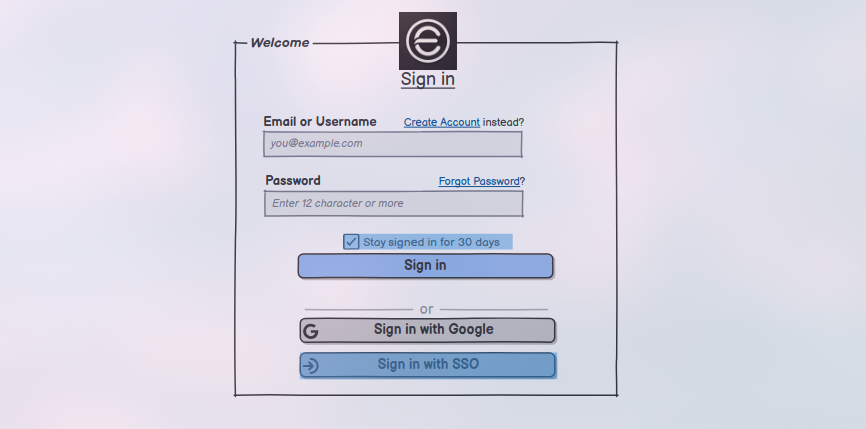
\includegraphics[width=1\textwidth]{Abbildungen/events/login.png}
    \caption{Login}
    \label{fig:login}
\end{figure}

\subsection{Events}
\subsubsection{Event-Feed}
\begin{figure}[H]
    \centering
    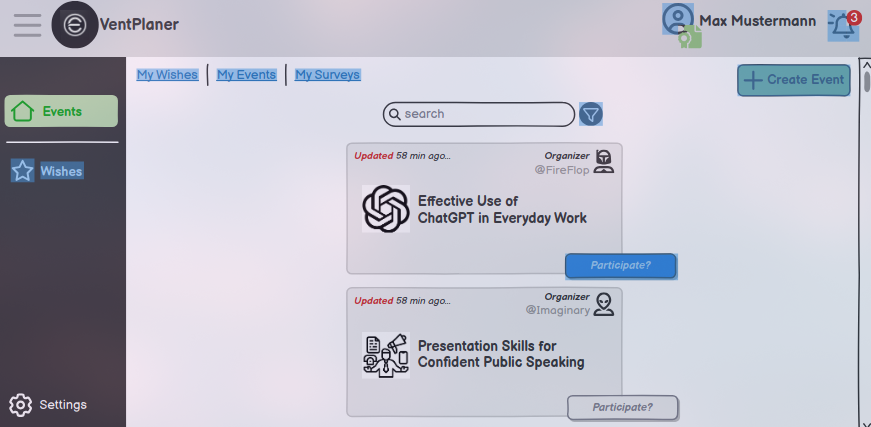
\includegraphics[width=1\textwidth]{Abbildungen/events/event_feed.png}
    \caption{Event-Feed}
    \label{fig:event_Feed}
\end{figure}

\subsubsection{Meine Events}
\begin{figure}[H]
    \centering
    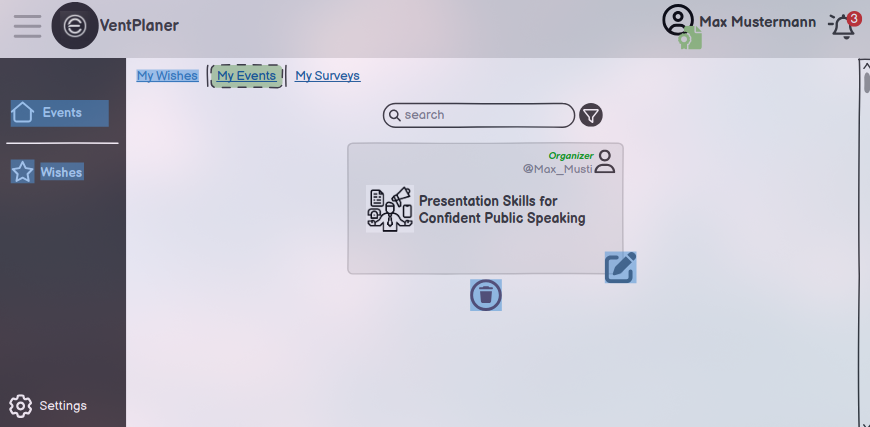
\includegraphics[width=1\textwidth]{Abbildungen/events/my_events.png}
    \caption{Meine Events}
    \label{fig:my_events}
\end{figure}

\subsubsection{Event erstellen}
\begin{figure}[H]
    \centering
    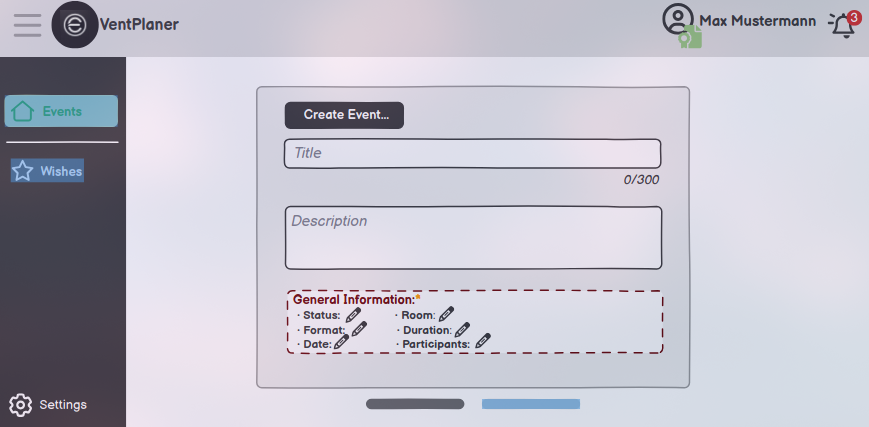
\includegraphics[width=1\textwidth]{Abbildungen/events/create_event.png}
    \caption{Event erstellen}
    \label{fig:create_event}
\end{figure}

\subsubsection{Umfrage erstellen}
\begin{figure}[H]
    \centering
    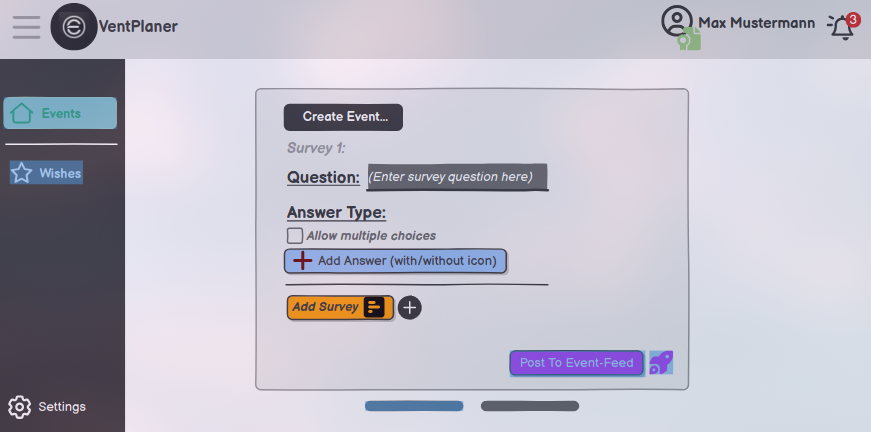
\includegraphics[width=1\textwidth]{Abbildungen/events/create_survey.png}
    \caption{Umfrage erstellen}
    \label{fig:create_survey}
\end{figure}

\subsubsection{Umfrage bearbeiten}
\begin{figure}[H]
    \centering
    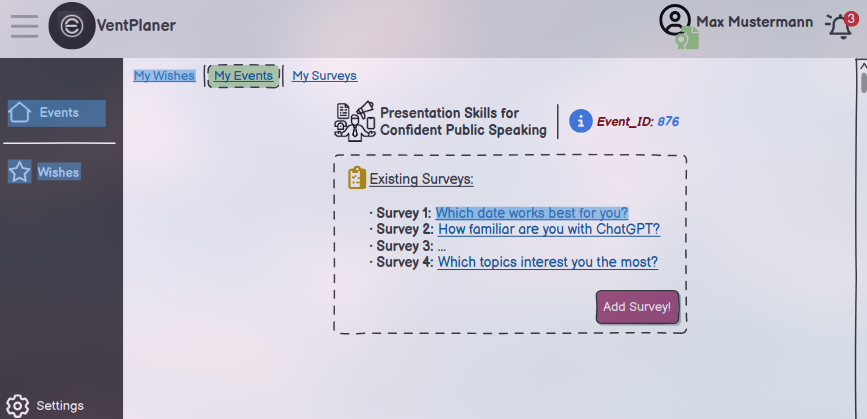
\includegraphics[width=1\textwidth]{Abbildungen/events/edit_survey.png}
    \caption{Umfrage bearbeiten}
    \label{fig:edit_survey}
\end{figure}

\subsubsection{Meine Umfragen}
\begin{figure}[H]
    \centering
    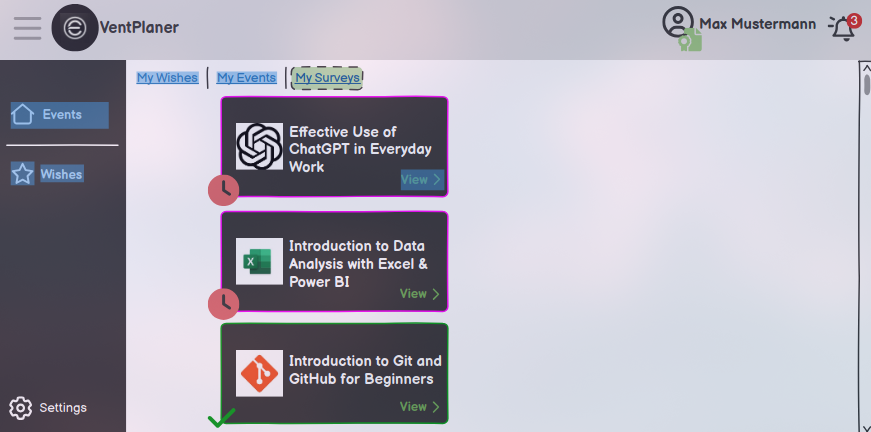
\includegraphics[width=1\textwidth]{Abbildungen/events/my_surveys.png}
    \caption{Meine Umfragen}
    \label{fig:my_survey}
\end{figure}

\subsubsection{Event bearbeiten}
\begin{figure}[H]
    \centering
    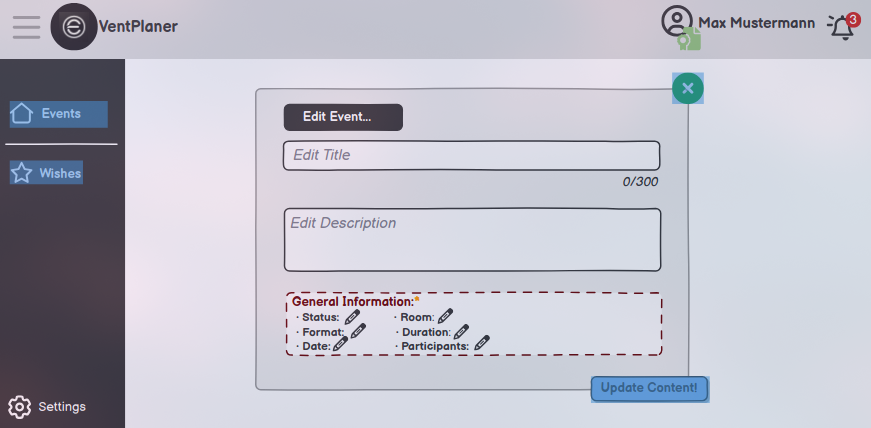
\includegraphics[width=1\textwidth]{Abbildungen/events/edit_event.png}
    \caption{Event bearbeiten}
    \label{fig:cedit_event}
\end{figure}

\subsubsection{Event löschen}
\begin{figure}[H]
    \centering
    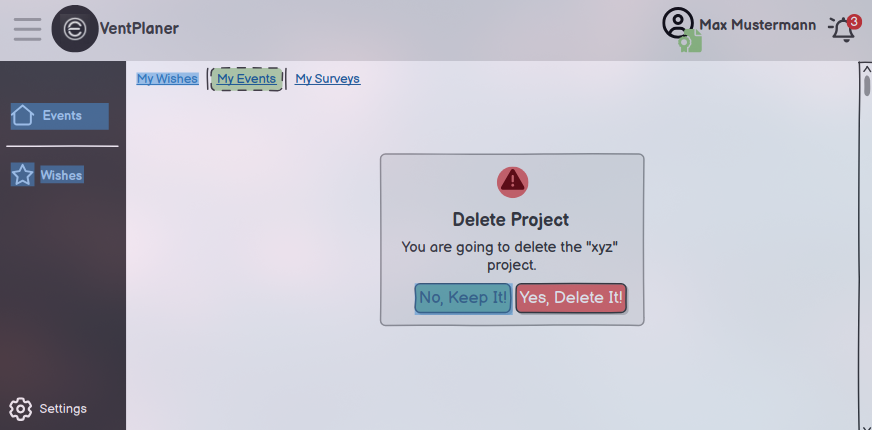
\includegraphics[width=1\textwidth]{Abbildungen/events/delete_event.png}
    \caption{Event löschen}
    \label{fig:delet_event}
\end{figure}

\subsection{Wünsche}
\subsubsection{Wünsche-Feed}
\begin{figure}[H]
    \centering
    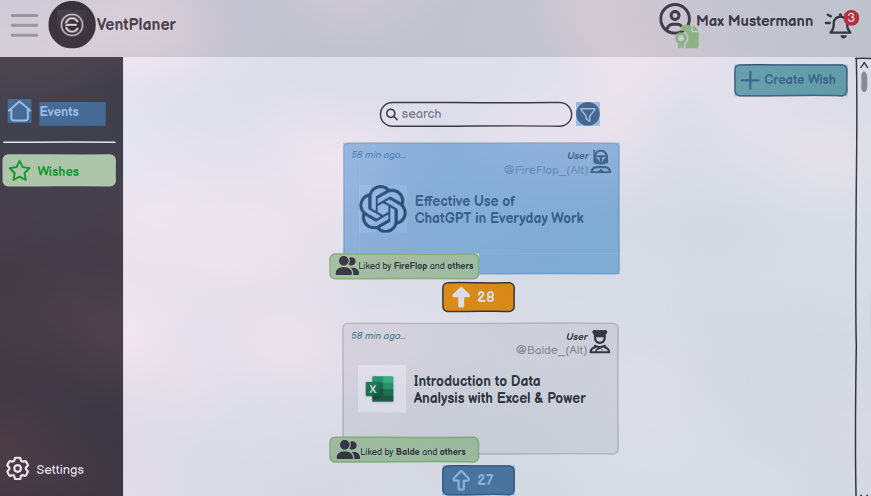
\includegraphics[width=1\textwidth]{Abbildungen/wishes/wishes-feed.png}
    \caption{Wünsche-Feed}
    \label{fig:wishes-feed}
\end{figure}

\subsubsection{Meine Wünsche}
\begin{figure}[H]
    \centering
    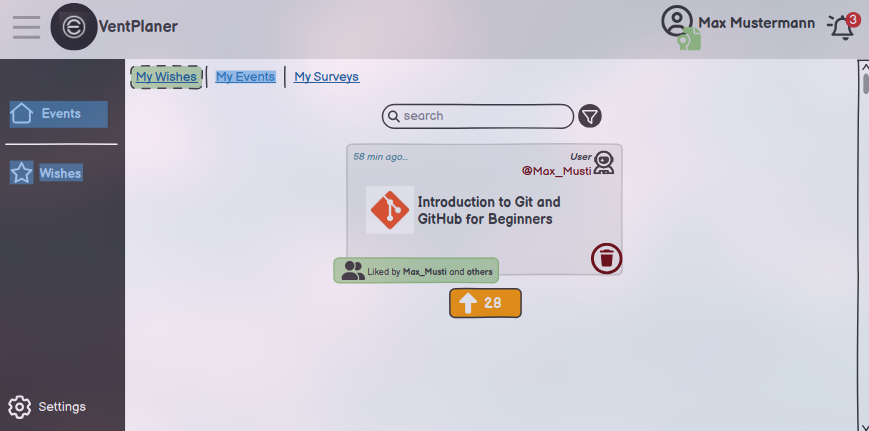
\includegraphics[width=1\textwidth]{Abbildungen/wishes/my-wishes.png}
    \caption{Meine Wünsche}
    \label{fig:my-wishes}
\end{figure}

\subsubsection{Wunsch erstellen}
\begin{figure}[H]
    \centering
    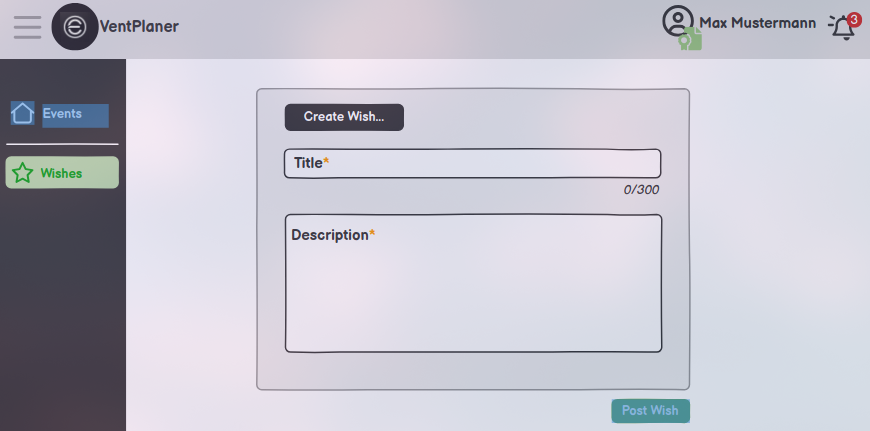
\includegraphics[width=1\textwidth]{Abbildungen/wishes/create_wish.png}
    \caption{Wunsch erstellen}
    \label{fig:create_wish}
\end{figure}

\newpage

%----------------------------------------------
% B Glossar
%----------------------------------------------

\printglossaries

\newpage

%----------------------------------------------
% B Literaturverzeichnis
%----------------------------------------------

\section{Literaturverzeichnis}

\end{document}
